%%%%%%%%%%%%%%%%%%%%%%%%%%%%%%%%%%%%%%%%%%%%%%%%%%%%%%%%%%%%%%%%%%%%%
% LaTeXTemplate: Project Titlepage Modified (v 0.1) by rcx
%
% Original Source: http://www.howtotex.com
% Date: February 2014
% 
% This is a title page template which be used for articles & reports.
% 
% This is the modified version of the original Latex template from
% aforementioned website.
% 
%%%%%%%%%%%%%%%%%%%%%%%%%%%%%%%%%%%%%%%%%%%%%%%%%%%%%%%%%%%%%%%%%%%%%%

\documentclass[12pt]{report}
\usepackage[a4paper]{geometry}
\usepackage[myheadings]{fullpage}
\usepackage{fancyhdr}
\usepackage{lastpage}
\usepackage{subcaption}

\usepackage{graphicx, wrapfig, subcaption, setspace, booktabs}
\usepackage[T1]{fontenc}
\usepackage[font=small, labelfont=bf]{caption}
\usepackage{fourier}
\usepackage[protrusion=true, expansion=true]{microtype}
\usepackage[english]{babel}
\usepackage{sectsty}
\usepackage{url, lipsum}

\usepackage{graphicx}
\usepackage{booktabs}
\usepackage{float}
\usepackage{amsmath}
\usepackage{amssymb}
\usepackage{url}
\usepackage{hyperref}
\usepackage{booktabs}
\usepackage{longtable}
\usepackage{url}
\usepackage{hyperref}
\usepackage{mathabx}
\usepackage{natbib}
\newcommand*\mean[1]{\overline{#1}}


\newcommand{\HRule}[1]{\rule{\linewidth}{#1}}
\onehalfspacing
\setcounter{tocdepth}{5}
\setcounter{secnumdepth}{5}

%-------------------------------------------------------------------------------
% HEADER & FOOTER
%-------------------------------------------------------------------------------
\pagestyle{fancy}
\fancyhf{}
\setlength\headheight{15pt}
\fancyhead[R]{Oana Vesa}
\fancyhead[L]{The Merger of Elliptical Galaxies}

\fancyfoot[R]{Page \thepage\ of \pageref{LastPage}}
%-------------------------------------------------------------------------------
% TITLE PAGE
%-------------------------------------------------------------------------------

\begin{document}

\title{ \normalsize \textsc{}
		\\ [2.0cm]
		\HRule{0.5pt} \\
		\LARGE \textbf{\uppercase{The Merger of Elliptical Galaxies}}
		\HRule{2pt} \\ [0.5cm]
		\normalsize \today \vspace*{5\baselineskip}}

\date{}

\author{ ASTR 506  \\
		Oana Vesa}

\maketitle
\tableofcontents
\newpage

%-------------------------------------------------------------------------------
% Section title formatting
\sectionfont{\scshape}
%-------------------------------------------------------------------------------

%-------------------------------------------------------------------------------
% BODY
%-------------------------------------------------------------------------------

\section*{Abstract}
\addcontentsline{toc}{section}{Abstract}

An investigation into the dynamics of two merging elliptical galaxies of $20000$ equally massed particles was conducted. Using equations of motion and a constant time-step leap-frog integration scheme (KDK, or Kick Drift Kick), two merger models were created. The first merger model had the two elliptical galaxies offset by an x-shift of $50$ and a y-shift of $20$. The second merger model had the two elliptical galaxies offset by an x-shift of $150$ and a y-shift of $20$. Both models were given an initial and opposite velocity kick in the x,y, and z direction of $\pm 0.2$, $\pm 0.1$, and $\pm 0.02$, repsectively.


\section*{Introduction}
\addcontentsline{toc}{section}{Introduction}

Studying the merger of galaxies is important for better understanding galaxy formation, which is a major area of research within astronomy.


Around the beginning of the Big Bang, the universe was pretty dense. At this time, galaxy mergers should have been frequent; thus, mergers should have played a major role on the influence of galaxy formation~\cite{mergers}. Galaxies are generally split into three broad categories: blue cloud, red sequence, and green valley. Galaxies within the blue cloud are typically galaxies undergoing star formation, such as spiral galaxies. Galaxies under the category of red sequence are galaxies that are dead and red, such as elliptical galaxies. The green valley is an in-between transition from blue cloud to red sequence. The Milky Way Galaxy is considered a green valley galaxy. The main question for astronomers is, what causes these galaxies to transition between categories?

Mergers are split into two categories: wet and dry. Wet mergers tend to occur between gas-rich galaxies and should trigger star formation; however, dry mergers occur between gas-poor galaxies and can quench star formation, producing more red galaxies~\cite{2008ApJ}. Both these scenarios are important in furthering our understanding of galaxy evolution. It is not always easy to observe galaxy mergers, however. Mergers last billions of years and it becomes difficult to constrain the progenitor and merging conditions~\cite{2008MNRAS}. 

Thus, n-body simulations are often utilized to recreate these processes to better study this phenomena. These n-body simulations utilize the same equations of motions used in this paper but also can account for the hydrodynamics of the systems and cosmology, which this report does not. By doing this, galaxy mergers can be somewhat accurately modeled to give astronomers more insight into the process.




\section*{Methods and Tests}
\addcontentsline{toc}{section}{Methods and Tests}
The dynamics of two merging elliptical galaxies of equally massed $20,000$ particles was investigated in Fortran. Two simulations were conducted. Each merging galaxy simulation was given some velocity kick to put the galaxies into orbit and given a different x and y position. The acceleration loop that governs the equations of motions was parallelized using OpenMP. Parallelization is an important tool for simulations with thousands of particles. It utilizes the cores of computing clusters to allocate resources so that multiple processes can be conducted simultaneously. This tremendously helps to not use a lot of a computer's CPU.

The main equation that governs the formation of the elliptical galaxies in these simulations is the equation of motion
\begin{equation} \label{eqn:equationofmotion}
    \vec{g} = -G \sum_{j=1, i \neq j}^{N} \frac{m_j \left( \vec{r_i} - \vec{r_j} \right)}{| \vec{r_i} - \vec{r_j} |^3},
\end{equation}
where $g$ is the gravitational acceleration, $G$ is the gravitational constant, $m_{j}$ is the mass of the $j^{th}$ particle, $N$ is the number of particles, and $\vec{r}$ is the position of the corresponding particles. This equation of motion is split up into three components for x,y, and z. Other important equations to take into account are the potential energy
\begin{equation}\label{eqn:potential_energy}
W = - \frac{1}{2} \sum_{i,j}^{N}
\frac{Gm_im_j}{| \vec{r_i} - \vec{r_j} |}    
\end{equation}
and the kinetic energy
\begin{equation}\label{eqn:kineticenergy}
K = - \frac{1}{2} \sum_{i}^N m_i \left( \vec{v_i} \right)^2.
\end{equation}

To avoid the particles having very large accelerations at small distances,a method called the Plummer softening, or force softening, was used. The Plummer softening also insures that the the simulation is stable. The Plummer softener is introduced by adding $\epsilon^2$ to the denominator of Equations~\ref{eqn:equationofmotion} and \ref{eqn:potential_energy} like so
\begin{equation} \label{eqn:plummersofteningeqnofmoiton}
\vec{g} = -G \sum_{j=1, i \neq j}^{N} \frac{m_j \left( \vec{r_i} - \vec{r_j} \right)}{(| \vec{r_i} - \vec{r_j} | + \epsilon^2 )^{3/2}}
\end{equation}
and 
\begin{equation}\label{eqn:potenitalsoftening}
    W = - \frac{1}{2} \sum_{i,j}^{N}
\frac{Gm_im_j}{| \vec{r_i} - \vec{r_j} | + \epsilon^2} .
\end{equation}

The integration scheme utilized was the constant time-step leap-frog (KDK or Kick Drift Kick) and direct summation to compute the accelerations. In the KDK integration scheme, the time steps are divided in half to ensure that the velocity and position vectors meet up simultaneously. KDK works by updating the velocity coordinates (called a kick), updating the positions coordinates afterwards (called a drift), updating acceleration,and then updating velocity again. 

The KDK integration was used due to the fact that the orbit does not drift as much as the other integration schemes; however, some drift was present in the formation of the first initial cloud of $20000$ particles.



\section*{Analytical Estimates}
\addcontentsline{toc}{section}{Analytical Estimates}


\begin{table}[h]
\begin{tabular}{@{}lcccc@{}}
\toprule
\multicolumn{5}{c}{\textbf{Particles Lost}} \\ \midrule
\multicolumn{1}{l|}{} & \multicolumn{1}{c|}{\textbf{Beginning of Merger}} & \multicolumn{1}{c|}{\textbf{During Merger}} & \multicolumn{1}{c|}{\textbf{After Merger}} & \multicolumn{1}{c|}{\textbf{Percentage Lost}} \\ \midrule
\multicolumn{1}{l|}{\textbf{Merger 1}} & $39656$ & $39633$ & $38712$ & \multicolumn{1}{c|}{$2.4\%$} \\ \midrule
\multicolumn{1}{c|}{\textbf{Merger 2}} & $39656$ & $38152$ & $35638$ & \multicolumn{1}{c|}{$10\%$} \\ \bottomrule
\end{tabular}
\caption{Number of Escaped Particles}
\label{tab:escapedparticles}
\end{table}


By defining a radius that encompasses most of the mass of the evolved elliptical galaxy or galaxies during a merger, the number of particles that have escaped from the system(s) can be determined. This can be seen in Table~\ref{tab:escapedparticles} above. The calculation of the number of particles that have escaped can be seen by creating a histogram of the system, binning out to a certain diameter, and then counting all of the particles in that diameter. 


\begin{figure}[h]
    \centering
    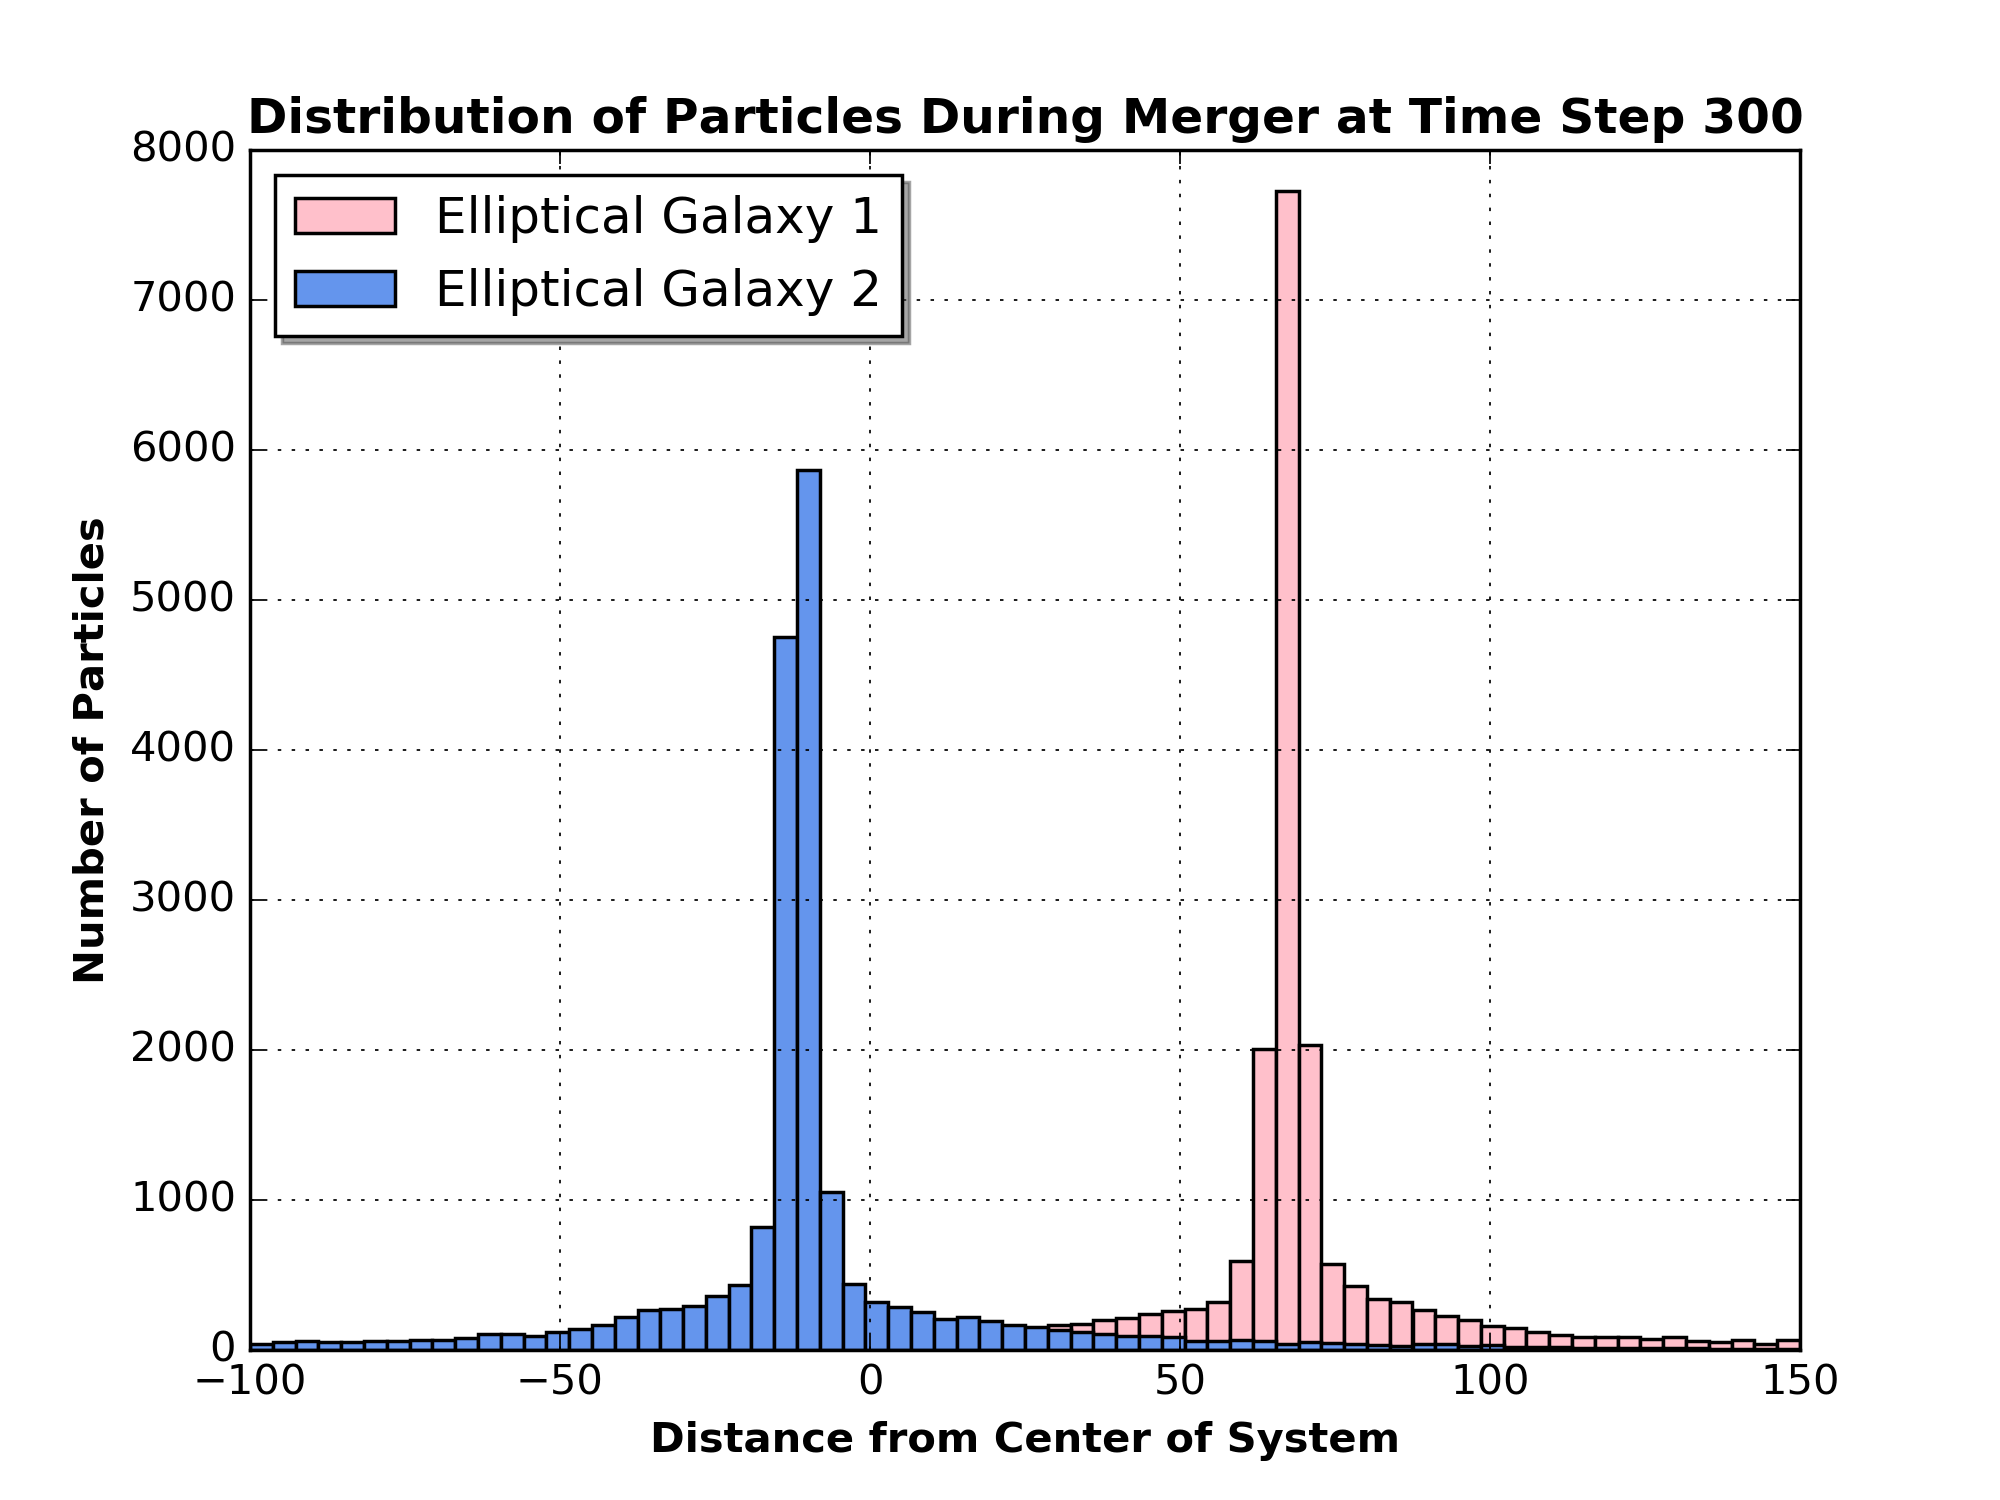
\includegraphics[width=\linewidth]{histogram_final_distributionofparticlesfromcenter_aftermerger.png}
    \caption{A histogram showing the distribution of particle after the merger in the first merger model.}
    \label{fig:histdist_merger1}
\end{figure}

For instance, as seen in Figure~\ref{fig:histdist_merger1} above, by doing this, one can account for a majority of the system without worrying about the number that are further out than this predetermined diameter surrounding the merger of the two systems. By summing up all of the particles in all the bins, the number of particles have escaped, $38712$ particles, can be determined. This number is seen in the first row of Table~\ref{tab:escapedparticles}.

The density of the elliptical galaxies was determined by defining a radius from the center of the system, where most of the mass was concentrated, to some distance out that still held a substantial amount of particles. Upon determining the radius steps for this, the following equation was used to determine the density
\begin{equation}\label{eqn:density_eqn}
    \rho = \frac{M}{V},
\end{equation}
where $\rho$ is the density of the system, $M$ is the mass of the system (and since all the particles have equal masses, the number of particles in that radius step was used instead), and $V$ is the volume of the system (which was approximated as $\frac{4}{3}\pi r^3$). Upon doing this, the following plots were created that show the initial density of the system and then the density of the two mergers.



Angular momentum was calculated by using the equation
\begin{equation}\label{eqn:angularmomentum_eqn}
    \vec{L} = \vec{r} \cross m\vec{v},
\end{equation}
where $\vec{L}$ is the angular momentum, $r$ is the position of all of the particles averaged, and $v$ is the velocity of all of the particles averaged. By doing so, the following plots were created that show the total angular momentum of the two mergers.



\section*{Results}
\addcontentsline{toc}{section}{Results}












\begin{figure}[H]
\centering 
    \begin{subfigure}[b]{.475\textwidth}
        \centering
        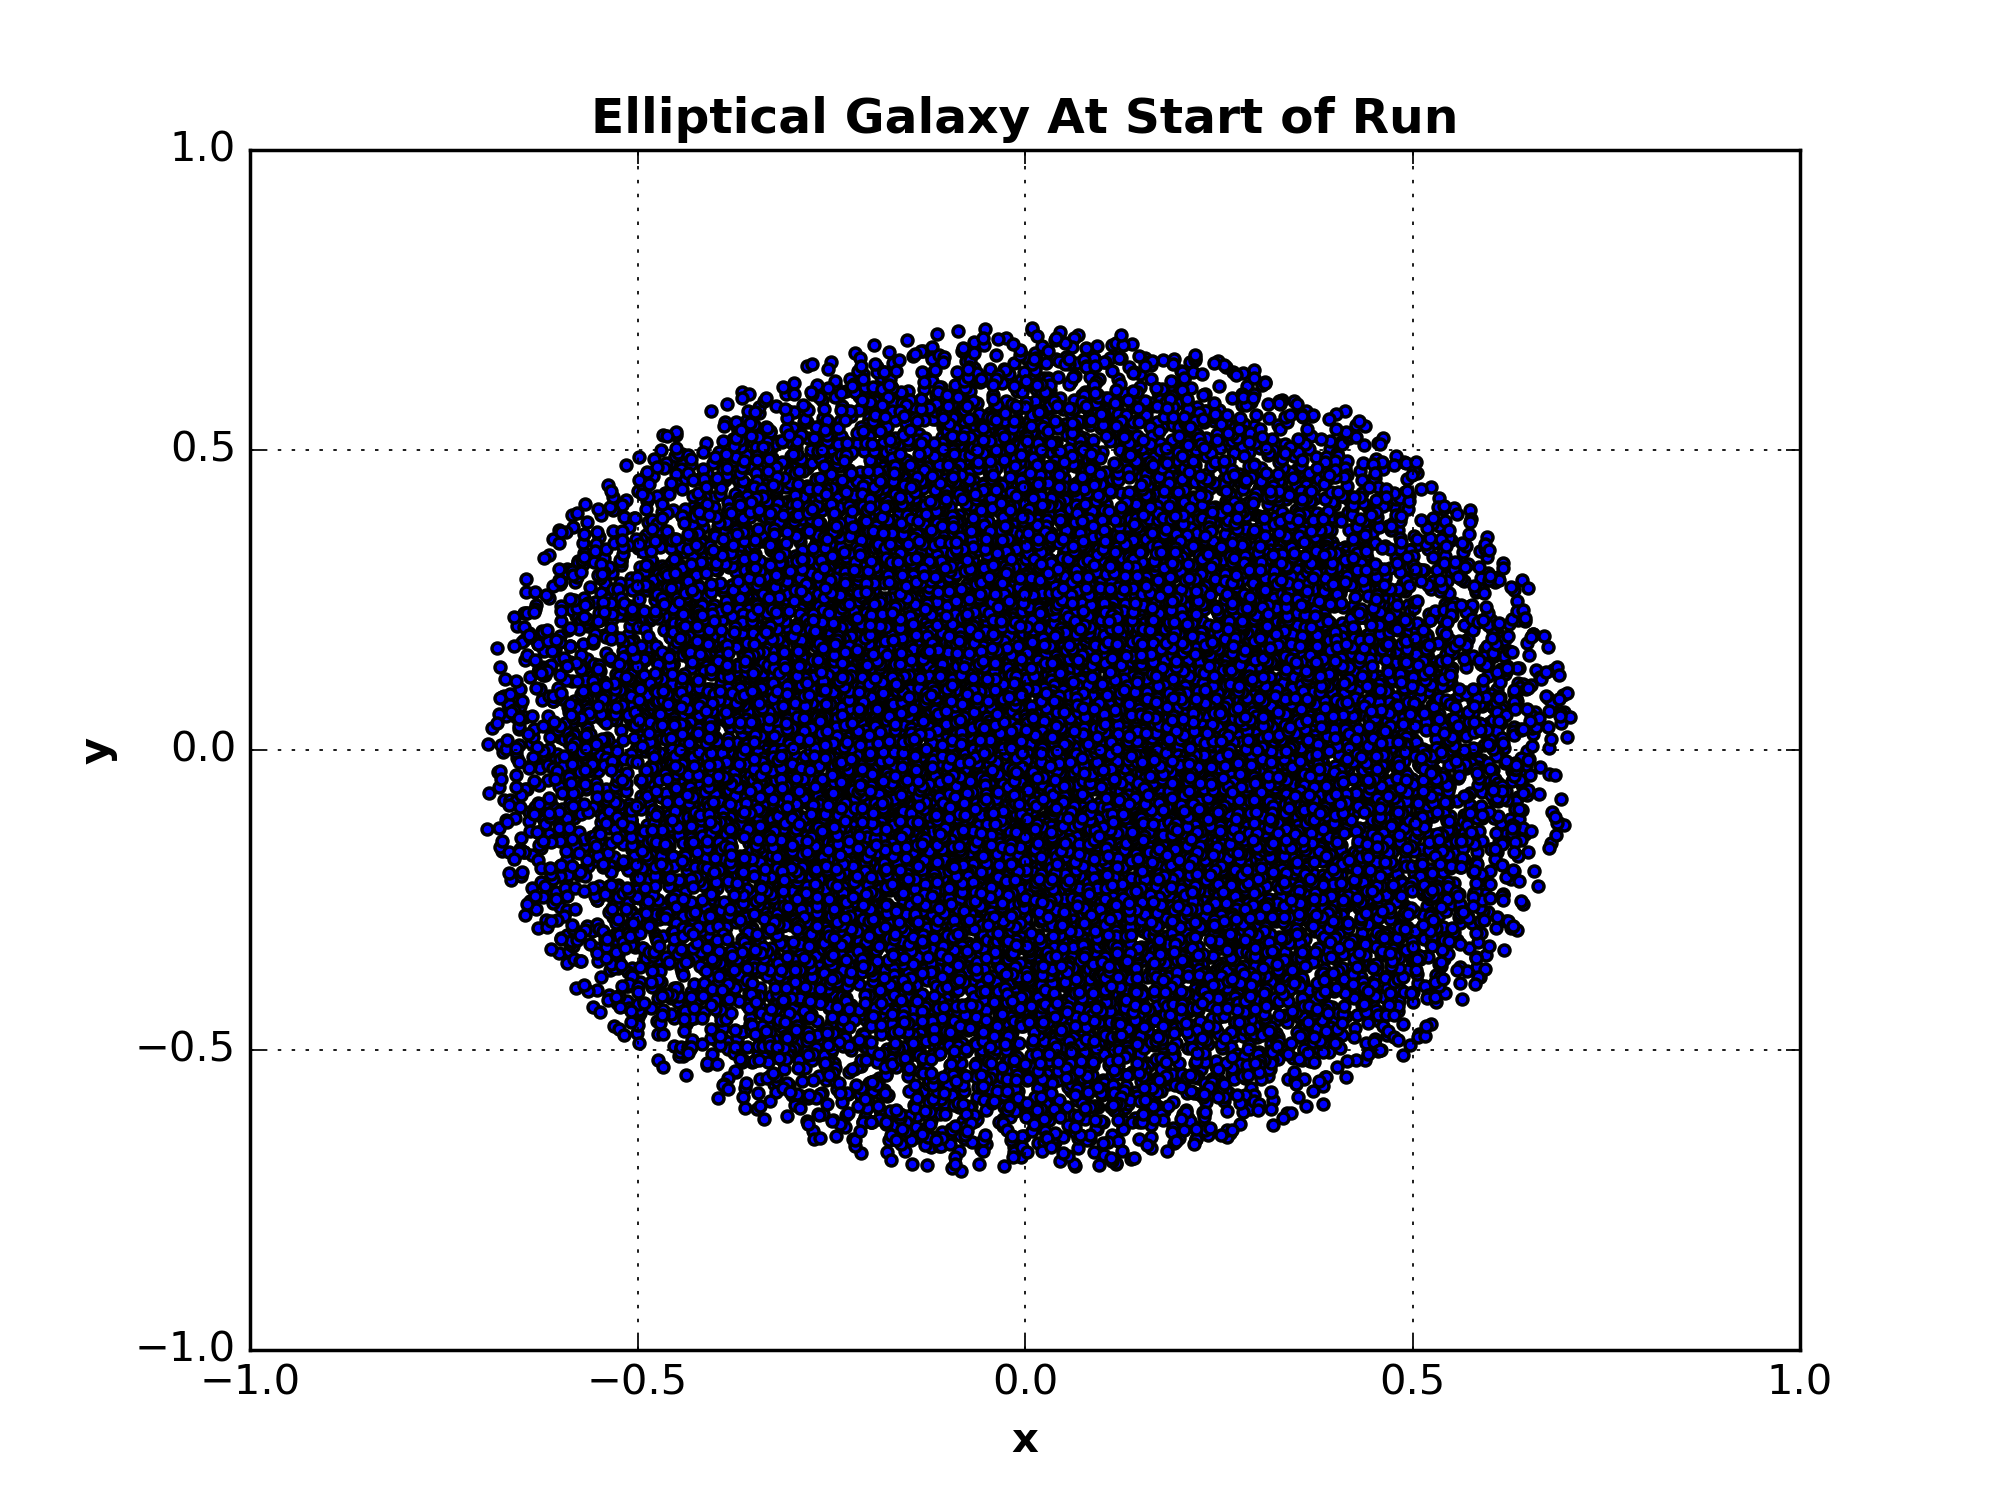
\includegraphics[width=\linewidth]{intiial_structure_of_cloud.png}
        \caption[]%
        {{\small This is the initial structure of the galaxy.}}
        \label{fig:pressurecomparisionfigure}
    \end{subfigure} %'
    \hfill
    \begin{subfigure}[b]{.475\textwidth}
        \centering
        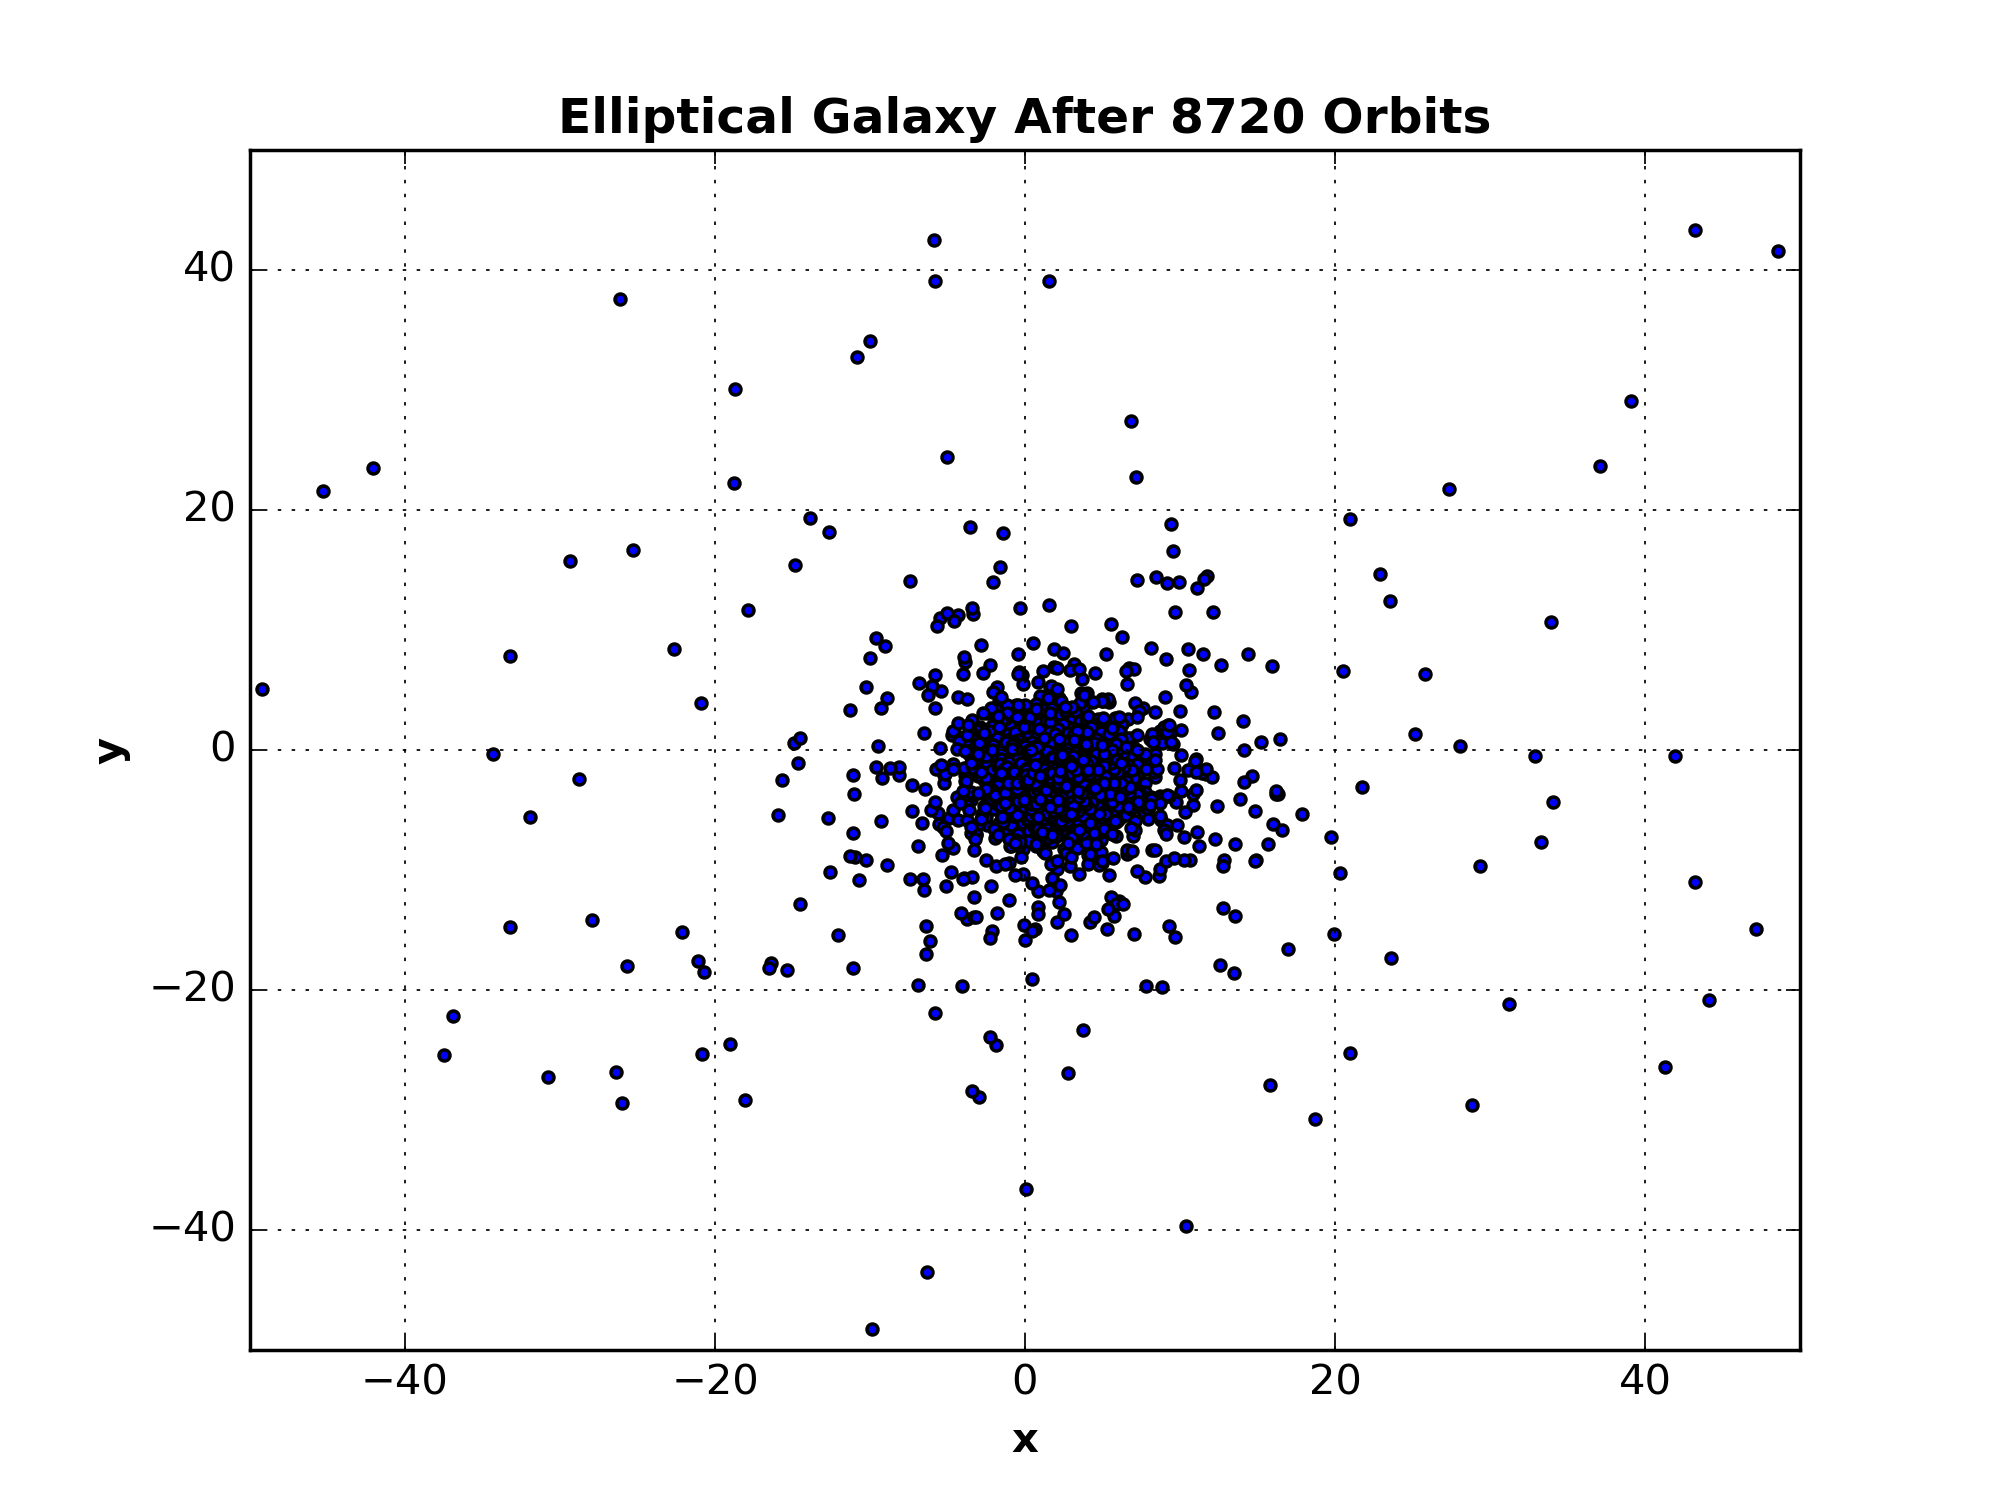
\includegraphics[width=\linewidth]{final_structure_of_cloud.png}
        \caption[]%
        {{\small This is the final structure of the galaxy.}}
        \label{fig:beta}
    \end{subfigure} %
    \caption[]
        {The plots above illustrate the structure of the elliptical galaxy of $20000$ particles with a scaled radius of $0.5$ after an evolution of $8720$ dynamical orbits.} 
        \label{fig:cloudstructure}
\end{figure}

As seen in Figure~\ref{fig:cloudstructure}, after $8720$ dynamical orbits, the cloud evolved and became larger. Some of the particles escaped the system, and the system slightly drifted to the right.


\begin{figure}[H]
\centering 
    \begin{subfigure}[b]{.475\textwidth}
        \centering
        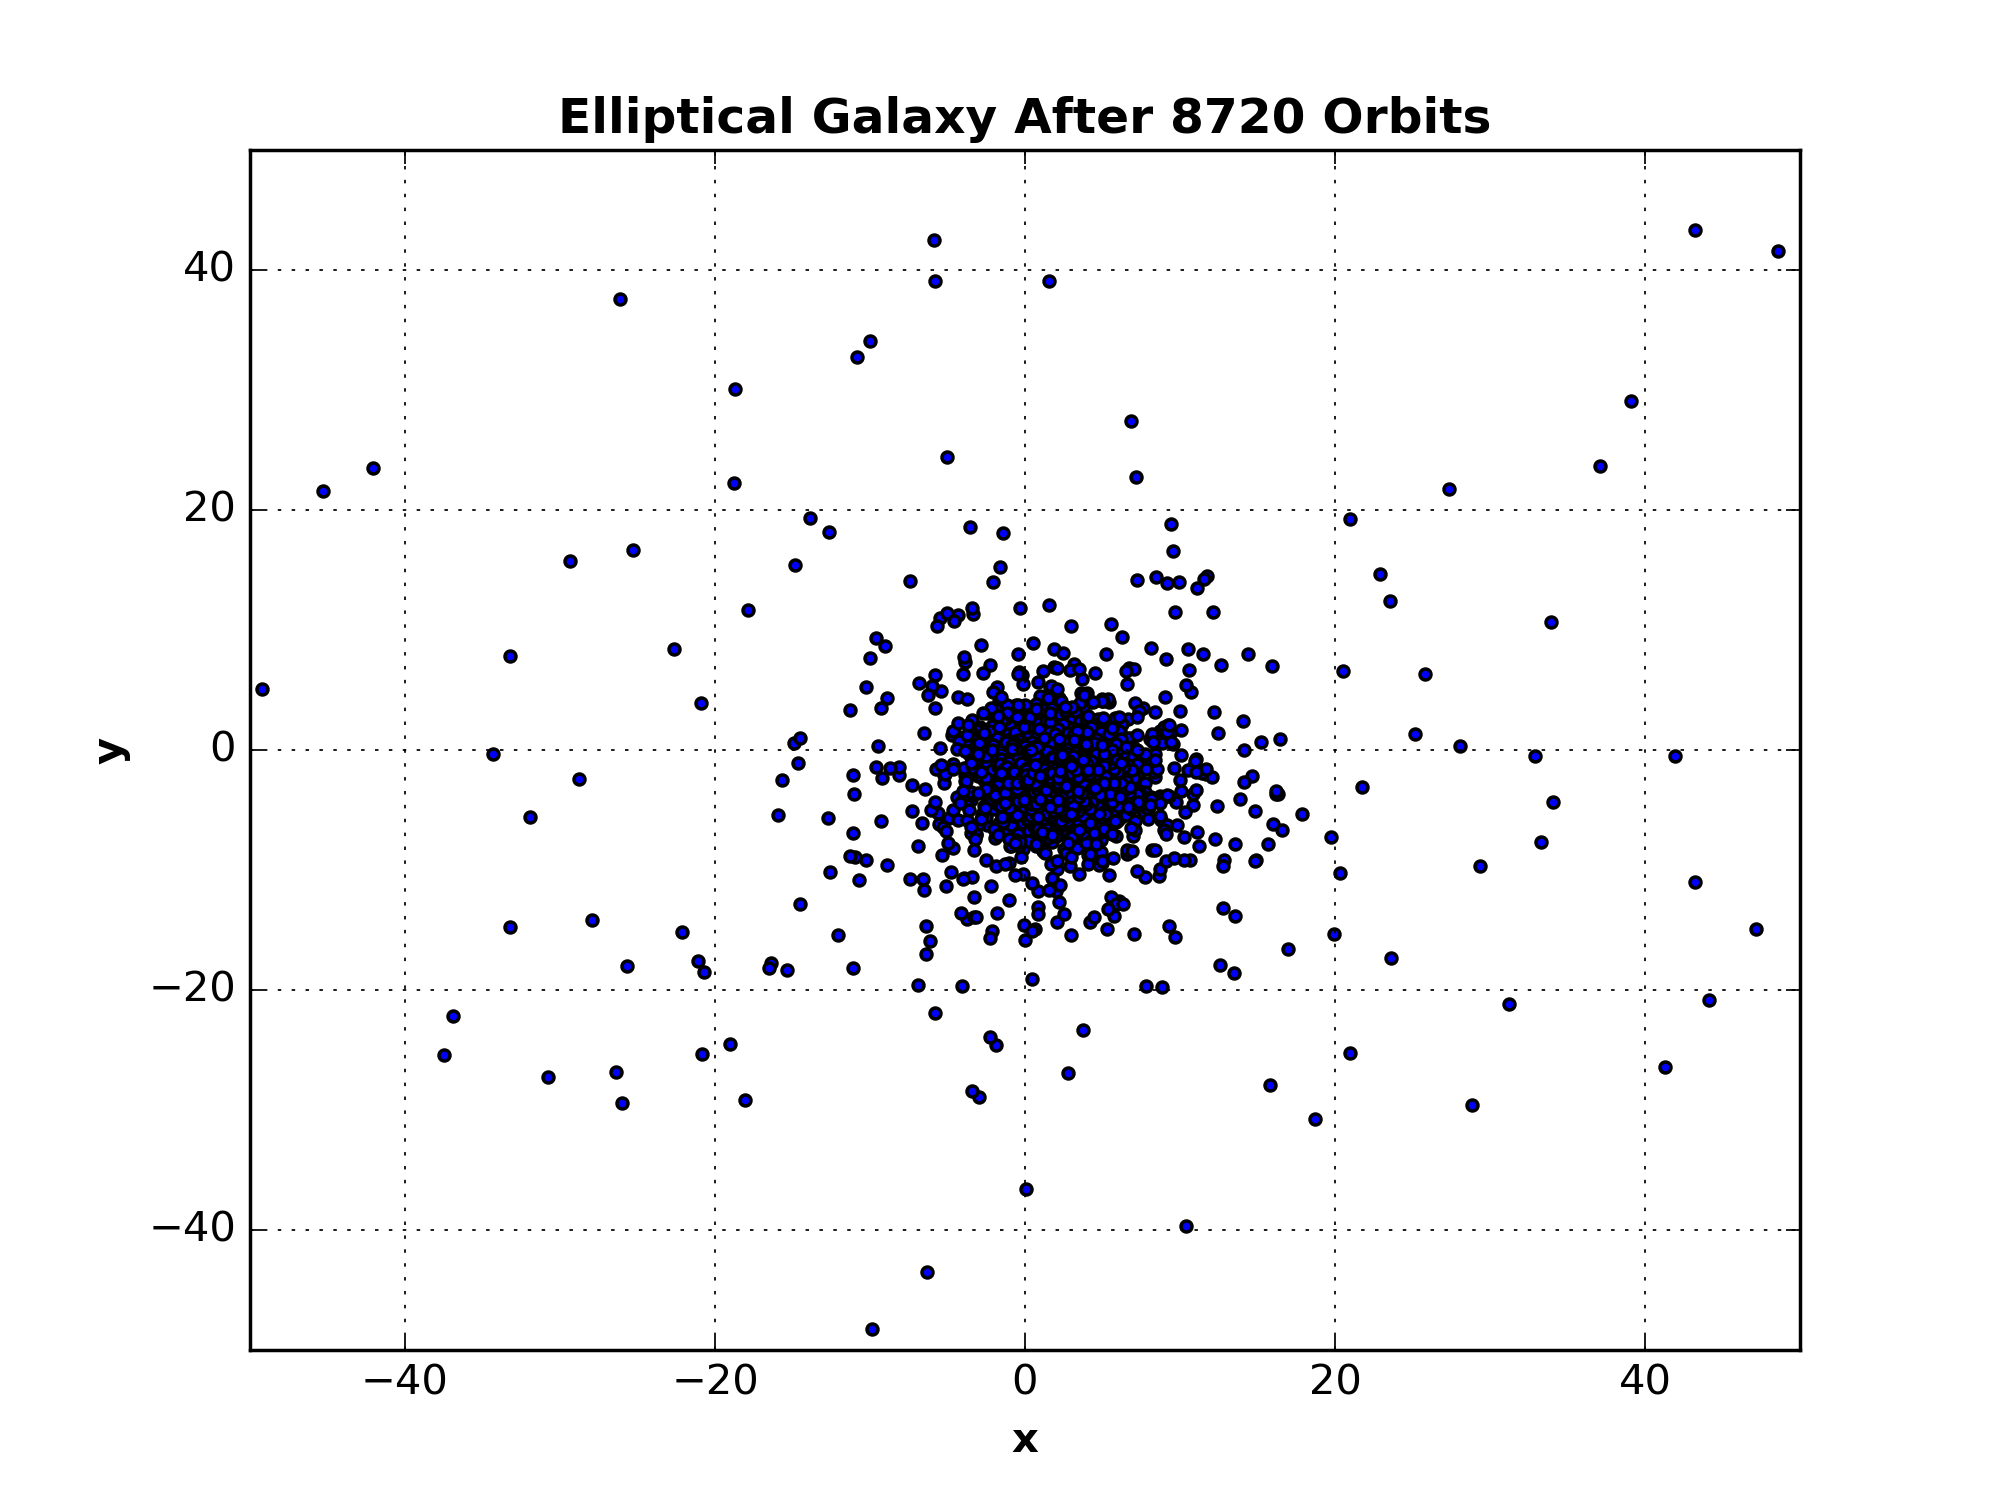
\includegraphics[width=\linewidth]{final_structure_of_cloud.png}
        \caption[]%
        {{}}
        \label{fig:pressurecomparisionfigure}
    \end{subfigure} %'
    \hfill
    \begin{subfigure}[b]{.475\textwidth}
        \centering
        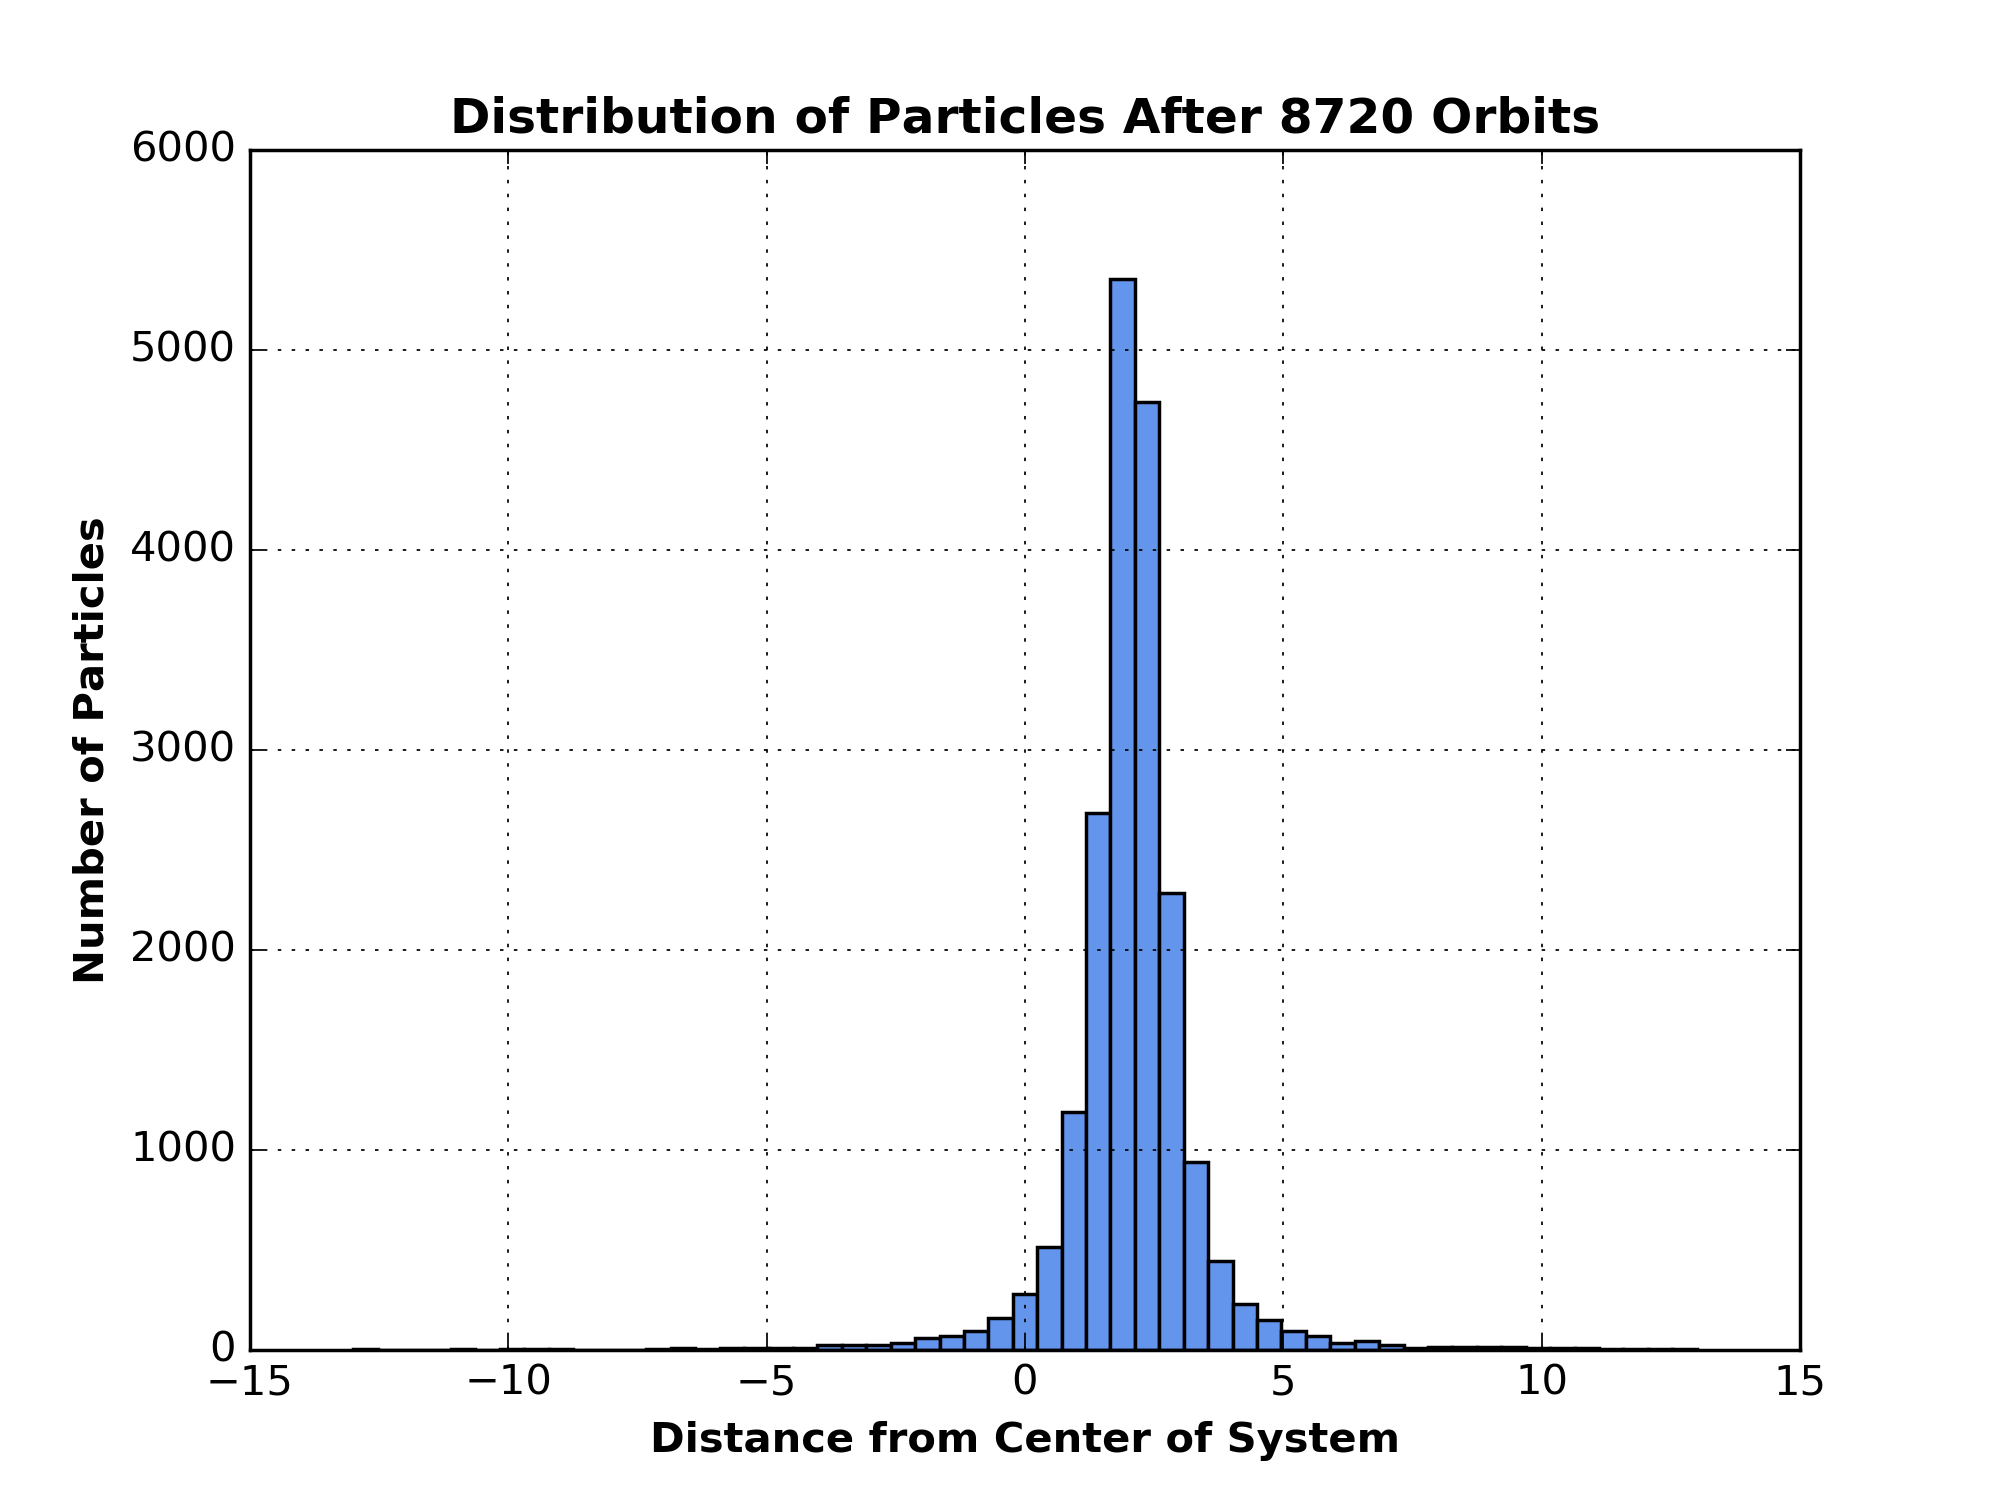
\includegraphics[width=\linewidth]{histogram_final_distributionofparticlesfromcenter.png}
        \caption[]%
        {{}}
        \label{fig:beta}
    \end{subfigure} %
    \caption[]
        {The plots above show the variation of various pressures (radiation,electron,total,gas,and nuclear) with optical depth.} 
        \label{fig:pressurefigure}
\end{figure}




\begin{figure}[H]
        \centering
        \begin{subfigure}[b]{0.48\textwidth}
            \centering
            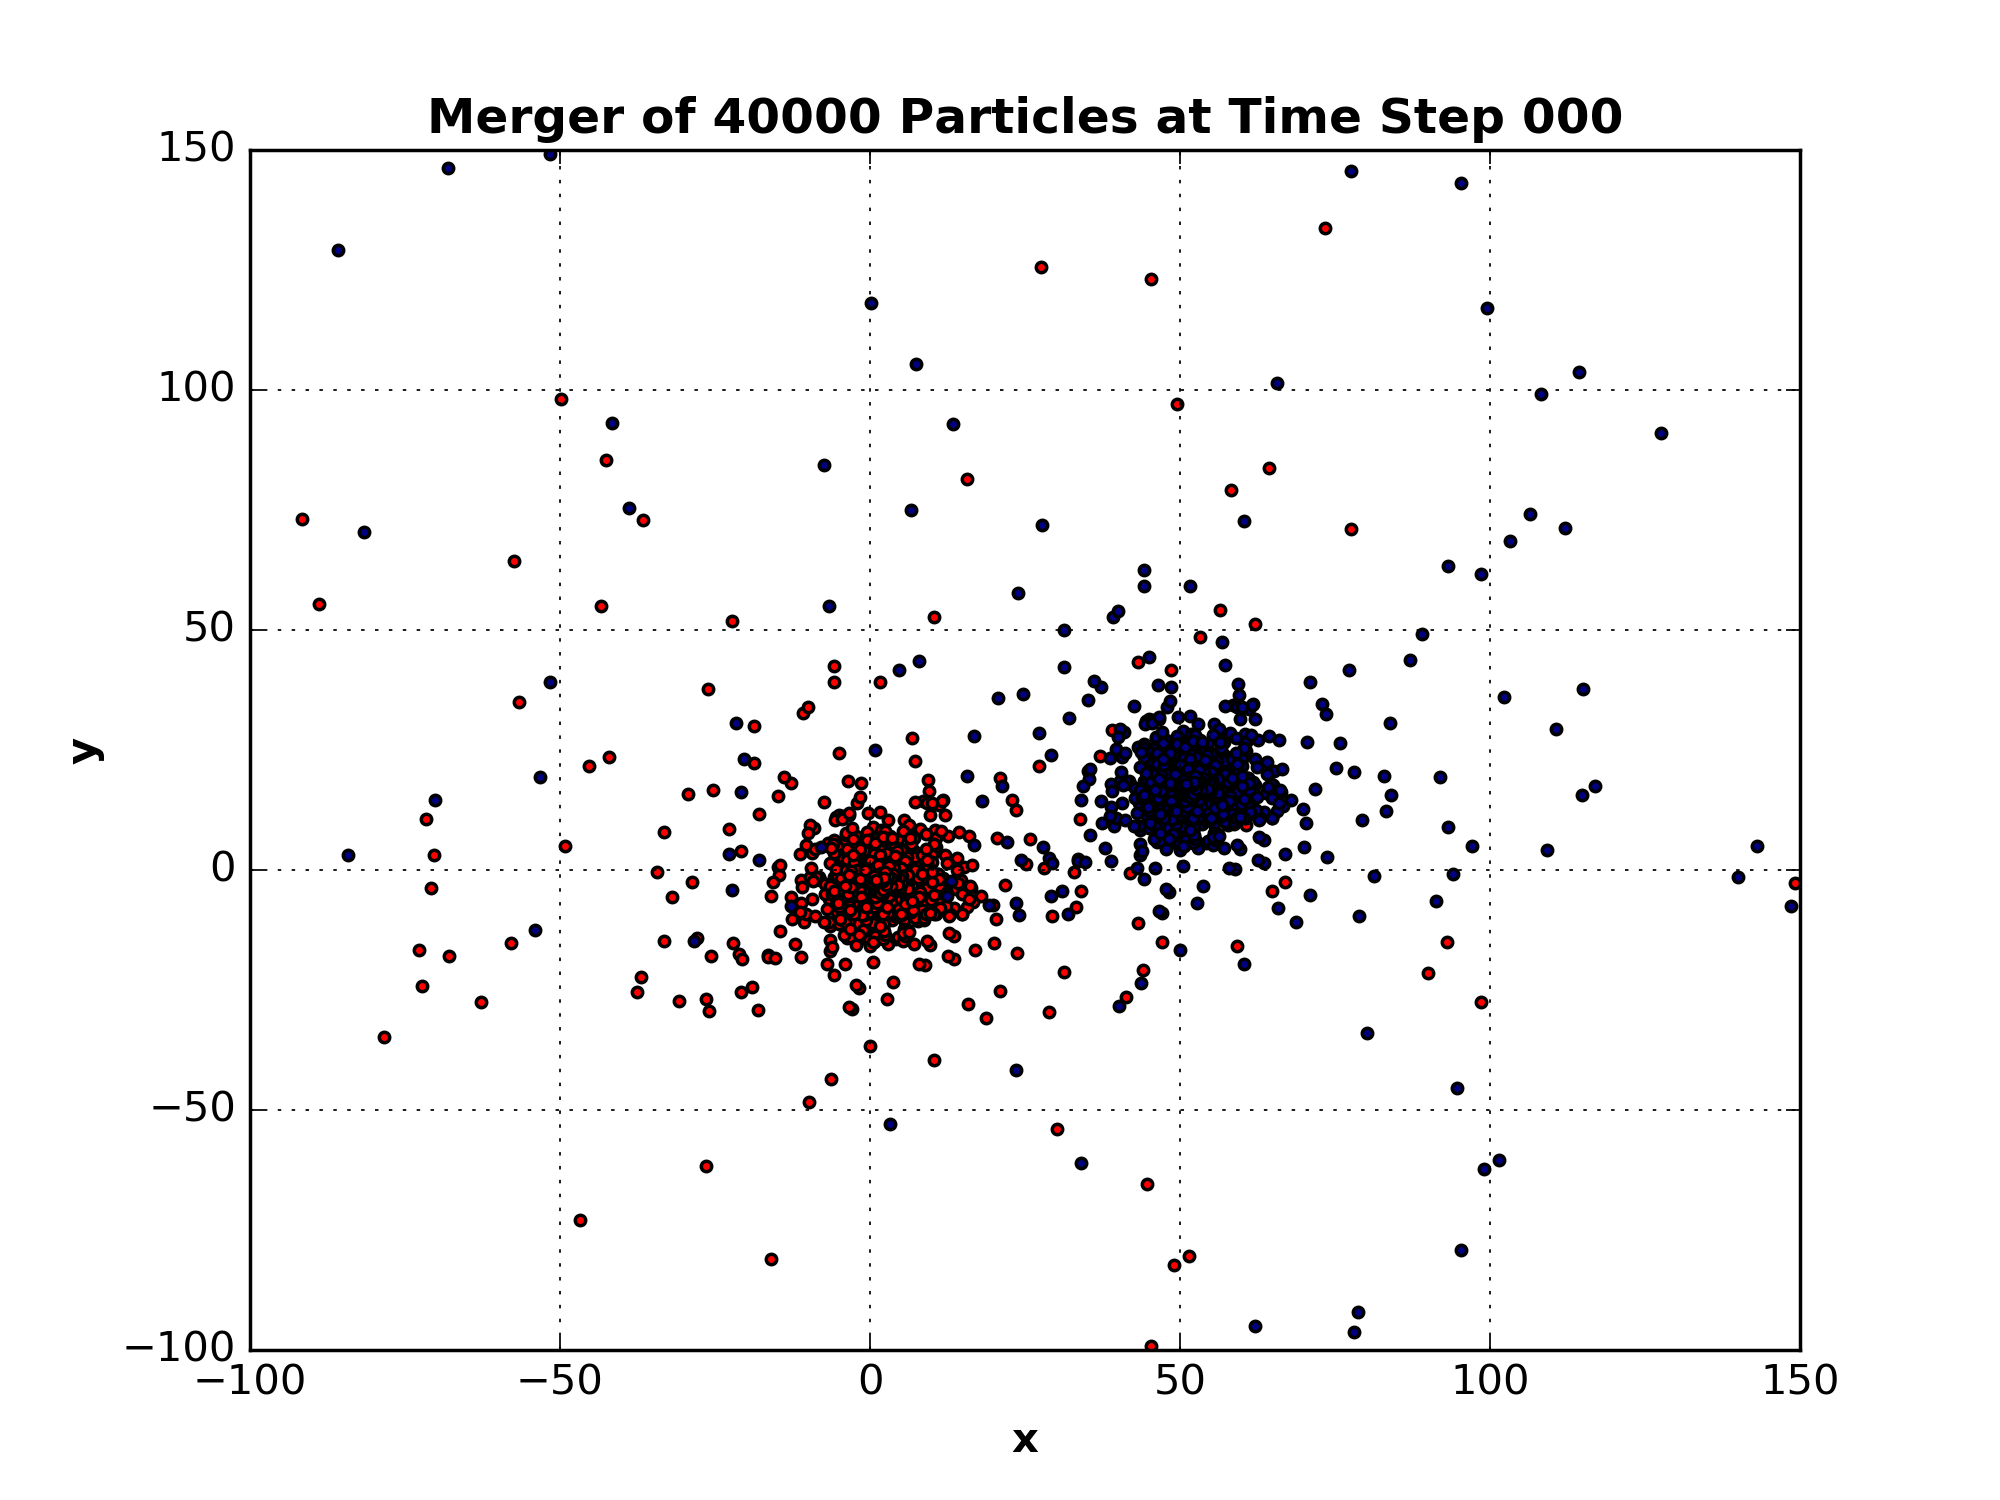
\includegraphics[width=\linewidth]{mergert000.png}
            \caption[]%
            {{\small The two elliptical galaxies separated by an x-shift of $50$ and y-shift of $20$.}}    
            \label{fig:merger1_t00}
        \end{subfigure}
        \hfill
        \begin{subfigure}[b]{0.48\textwidth}  
            \centering 
            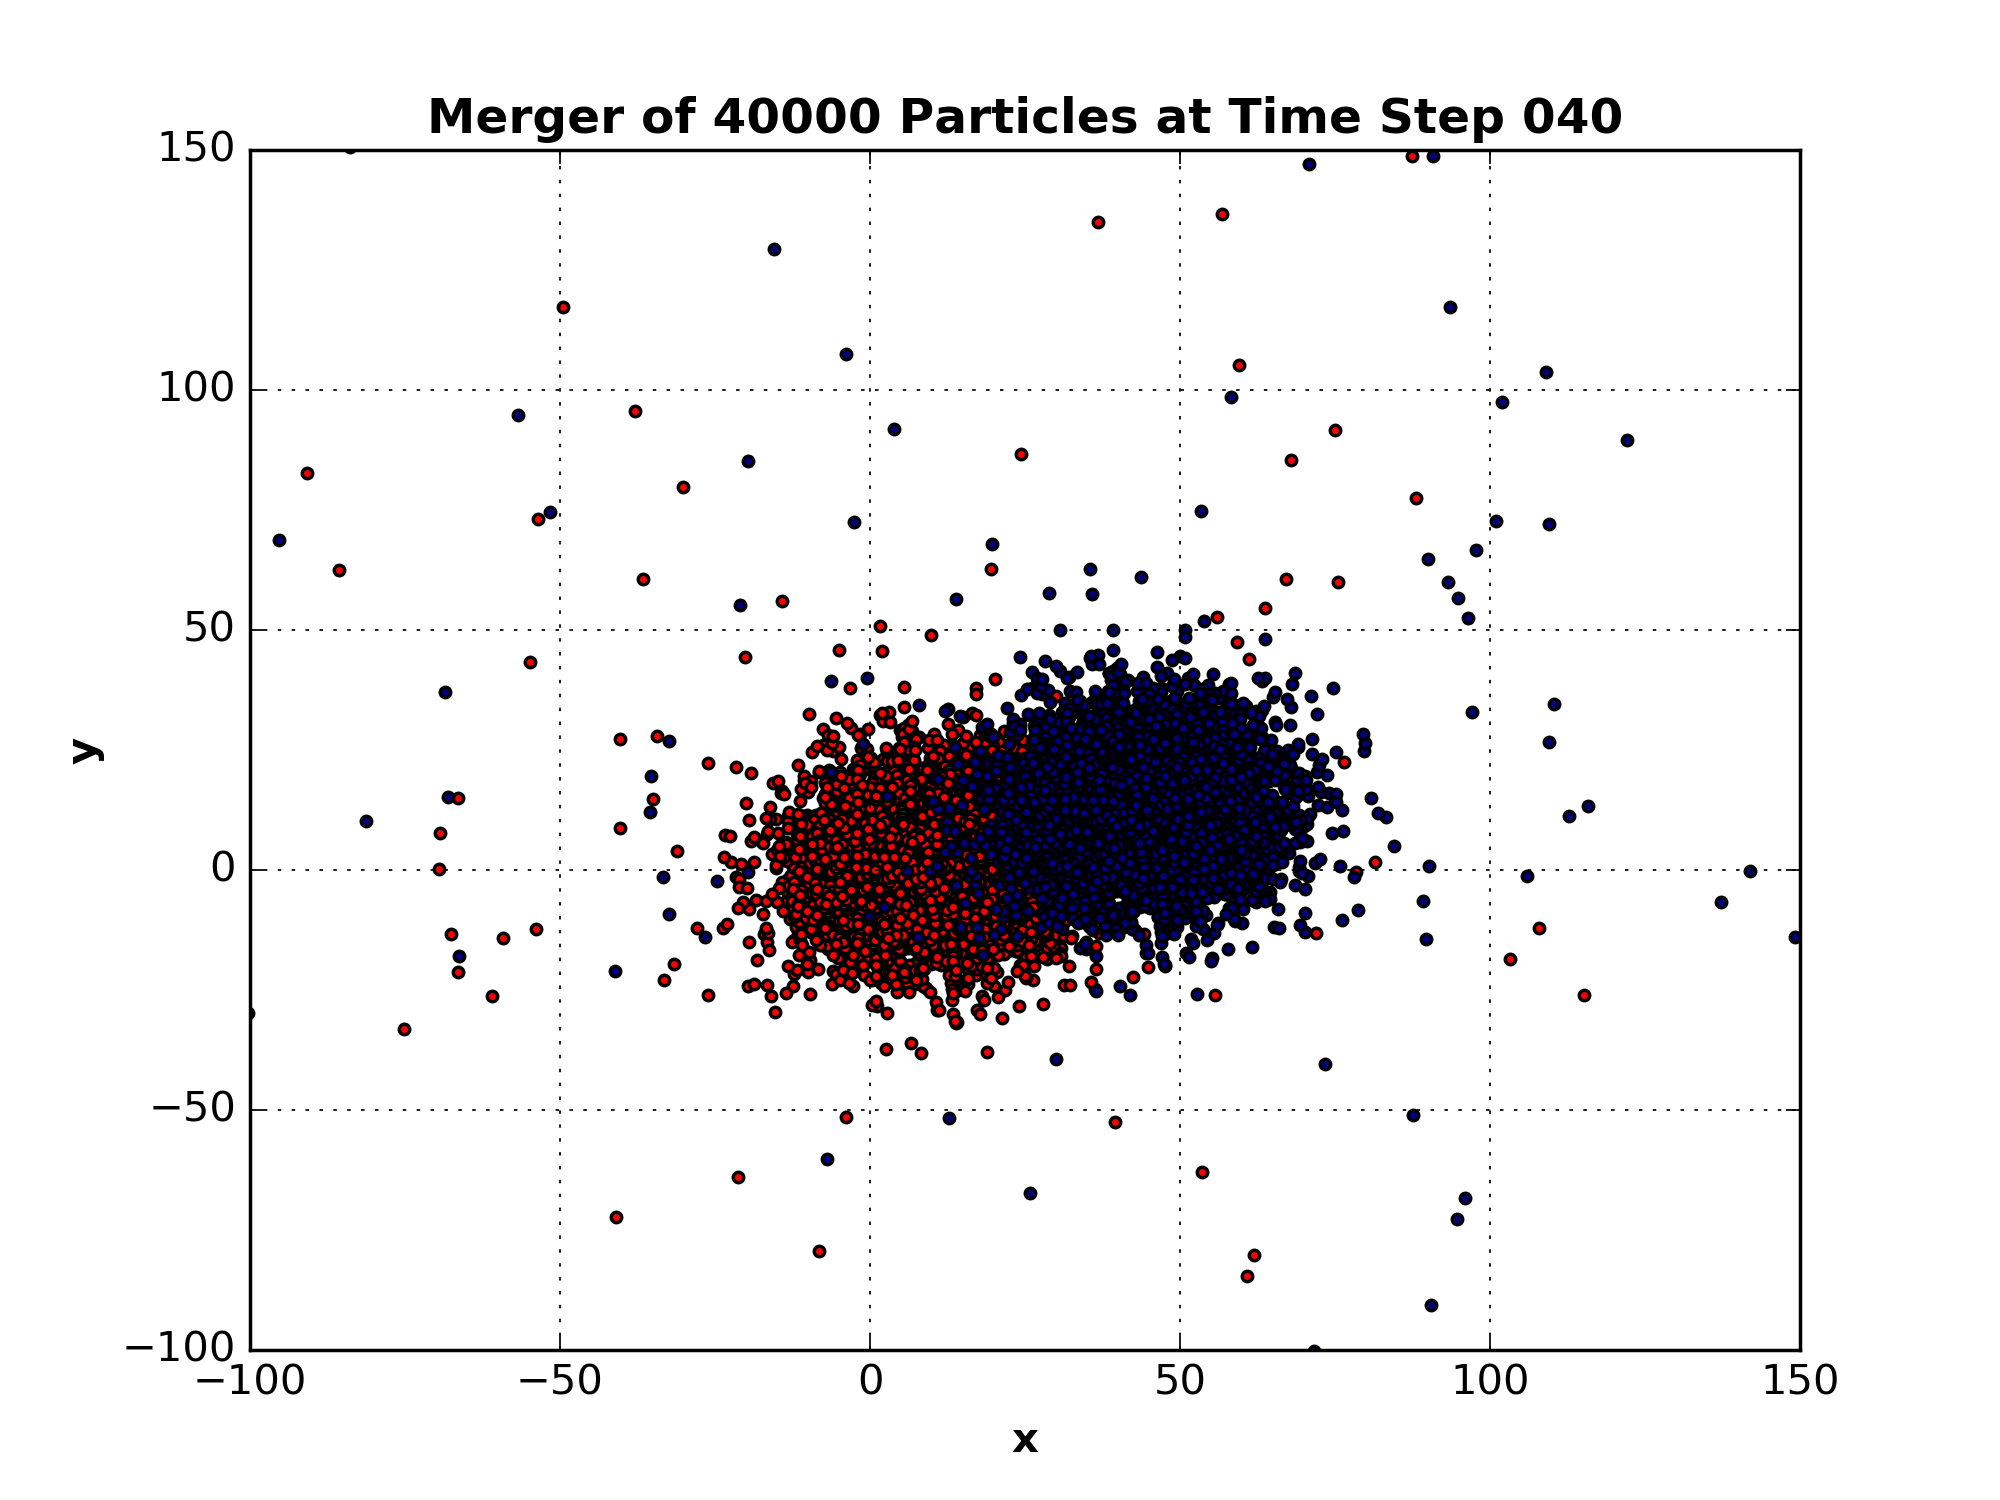
\includegraphics[width=\linewidth]{mergert040.png}
            \caption[]%
            {{\small The initial merging of the two elliptical galaxies at a time step of $040$.}}    
            \label{fig:merger1_t040}
        \end{subfigure}
        \vskip\baselineskip
        \begin{subfigure}[b]{0.48\textwidth}   
            \centering 
            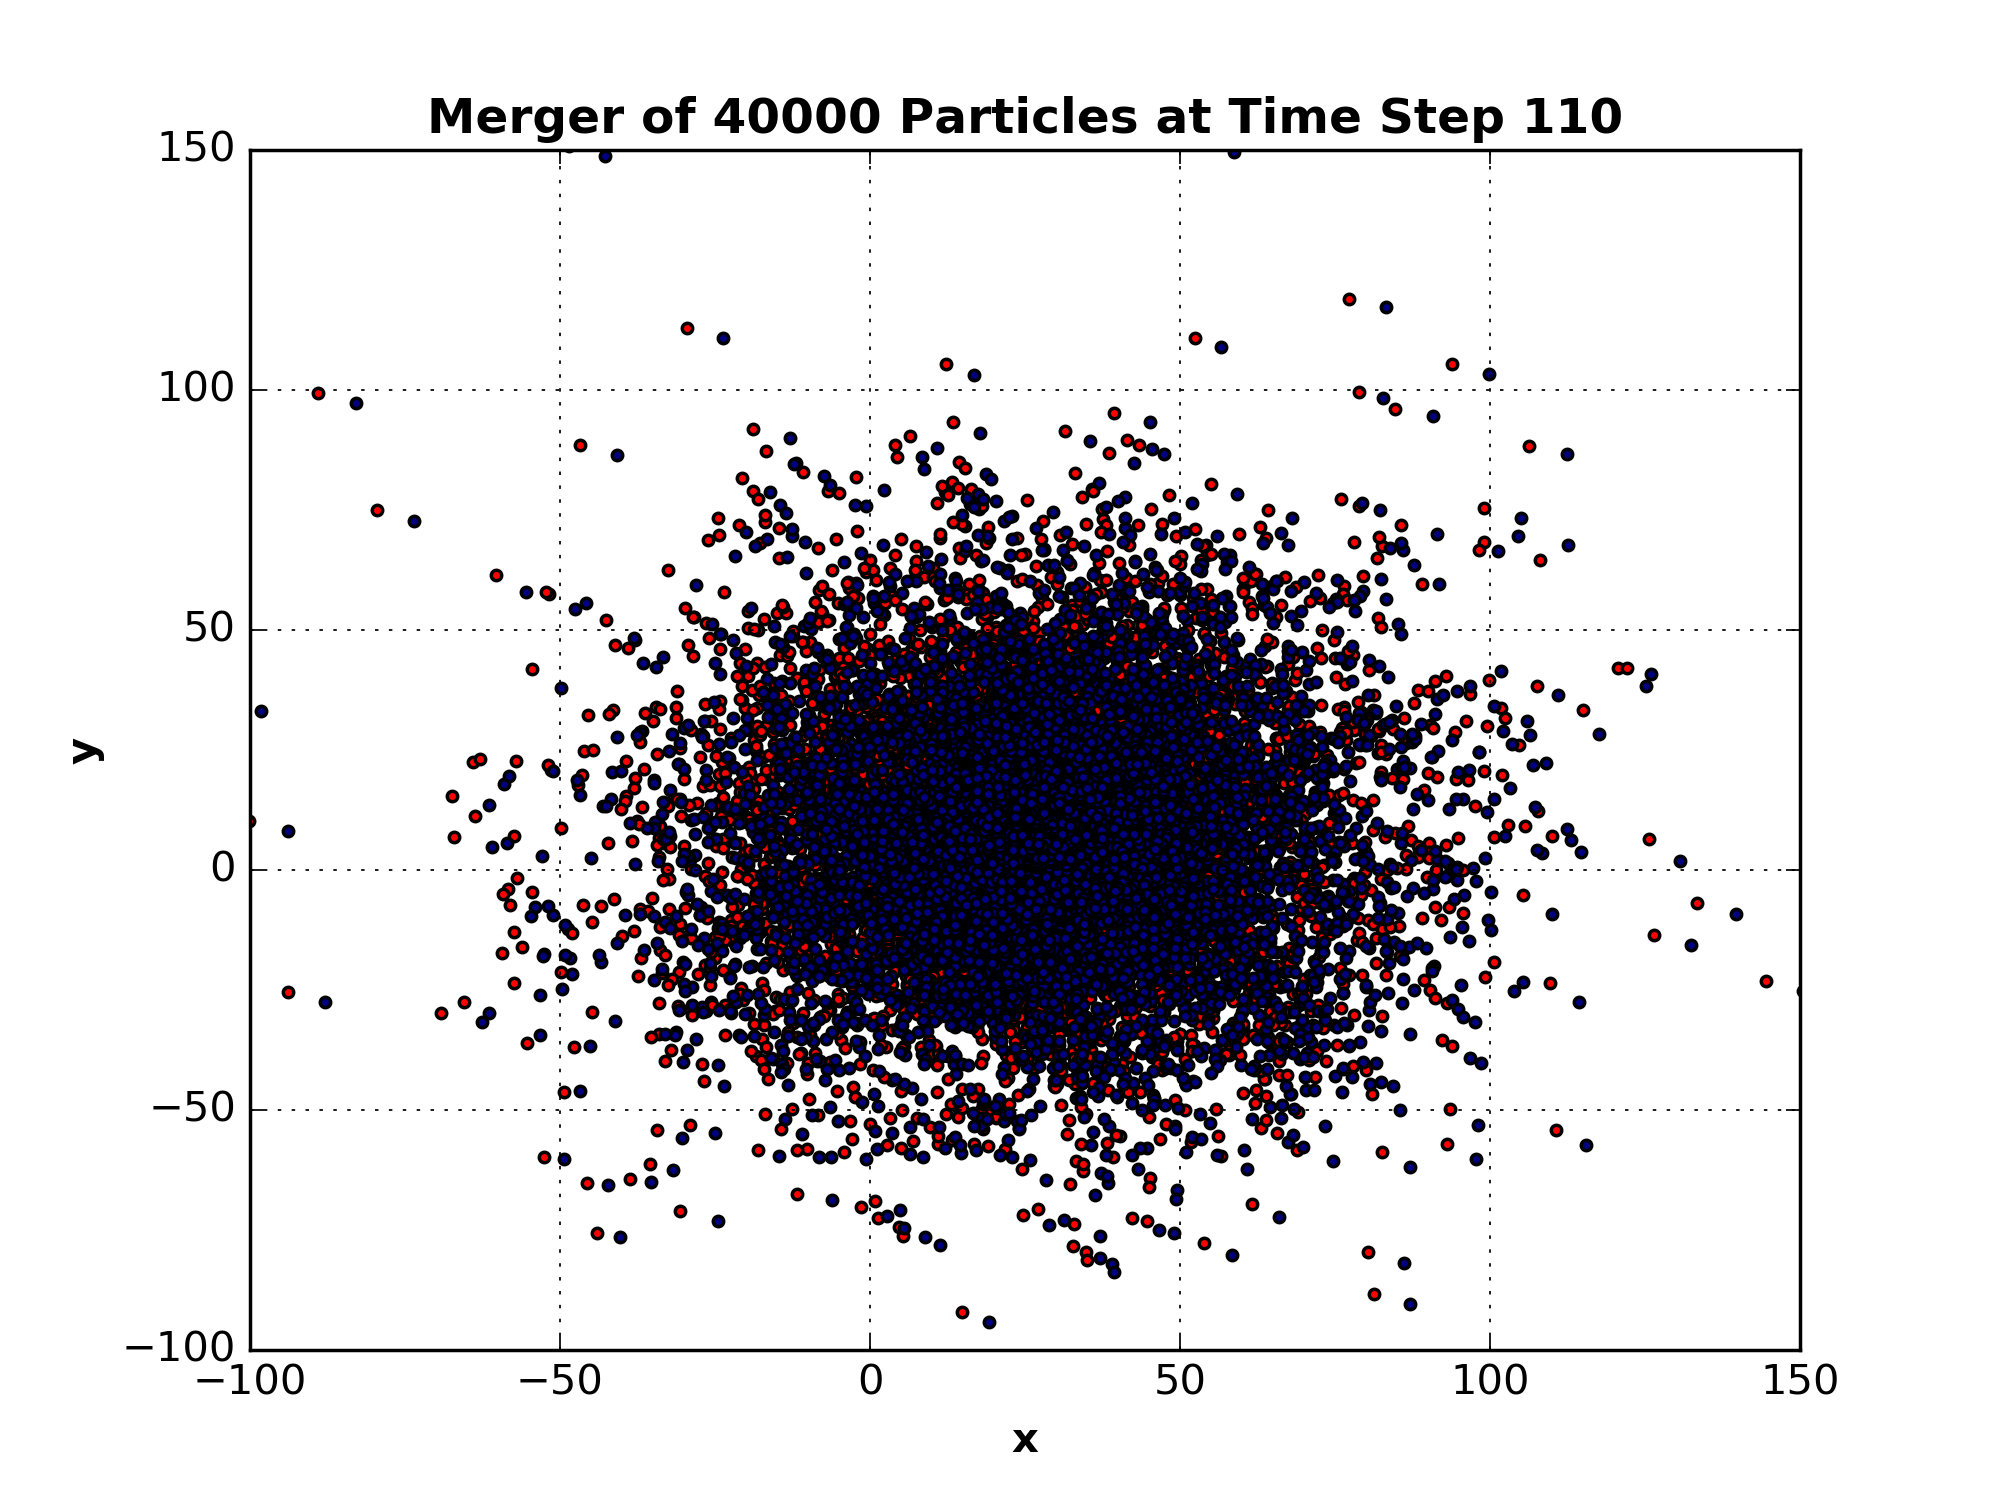
\includegraphics[width=\linewidth]{mergert110.png}
            \caption[]%
            {{\small The two elliptical galaxies completely merged at a time step of $110$.}}    
            \label{fig:merger1_t110}
        \end{subfigure}
        \quad
        \begin{subfigure}[b]{0.48\textwidth}   
            \centering 
            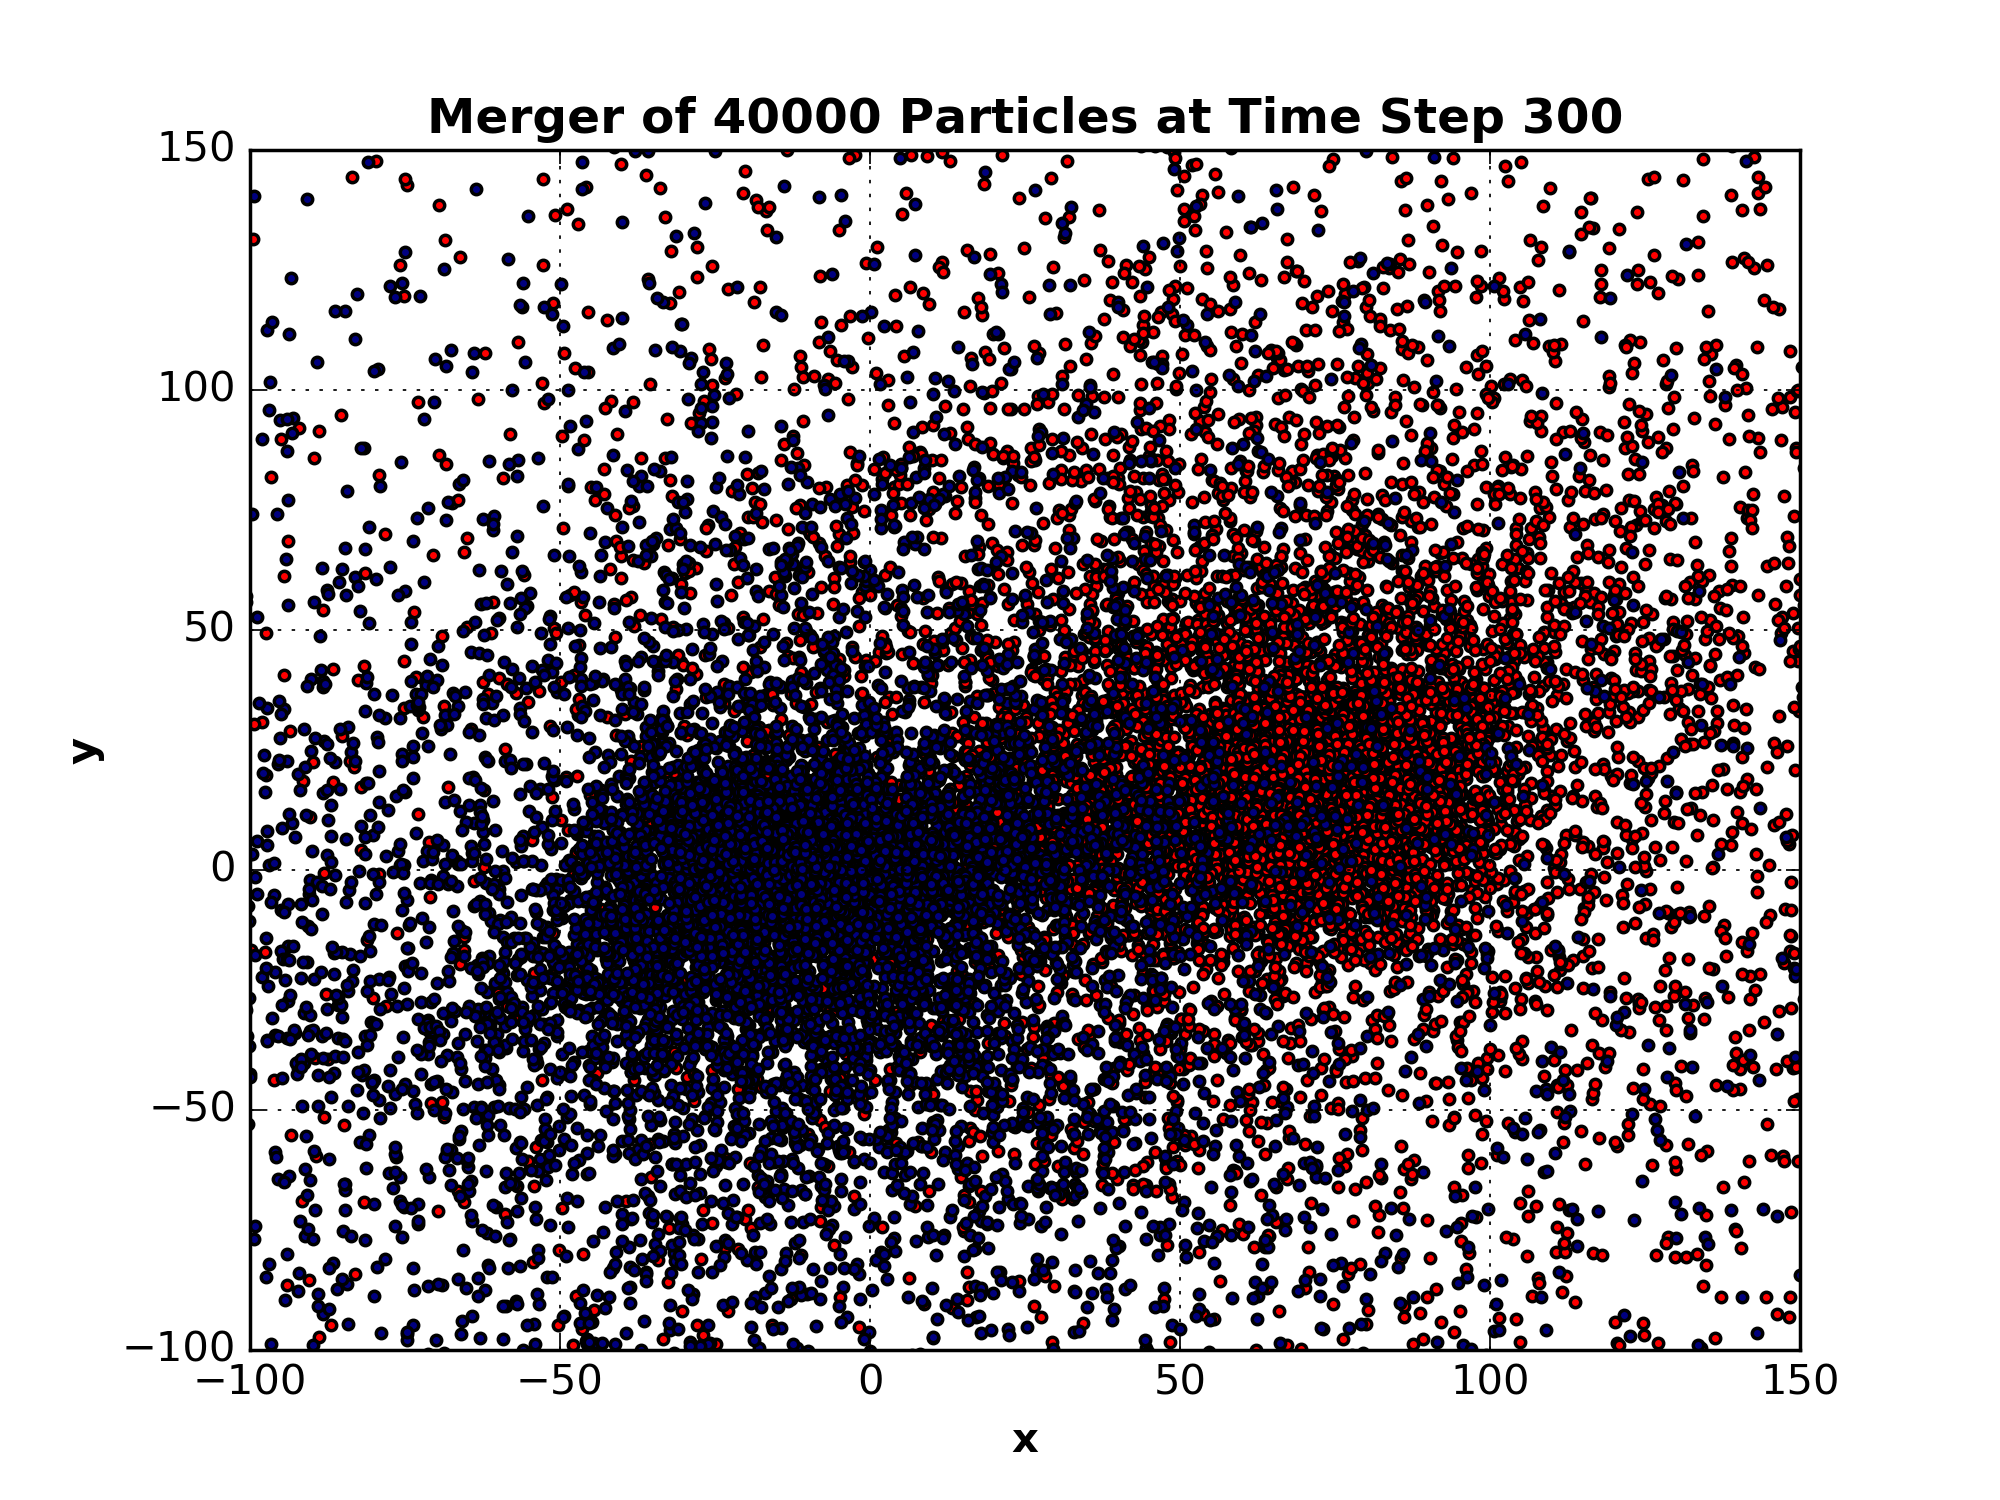
\includegraphics[width=\textwidth]{mergert300.png}\
            \caption[]%
            {{\small The two elliptical galaxies after the merger at a time step of $300$.}}
            \label{fig:merger1_t300}
        \end{subfigure}
        \caption[]
        {The plots above illustrate the first merger of two clouds of $20000$ particles each at different time steps.}
        \label{fig:merger1}
    \end{figure}
    
The energy of the first merger is illustrated below.

\begin{figure}[H]
\centering 
    \begin{subfigure}[b]{.475\textwidth}
        \centering
        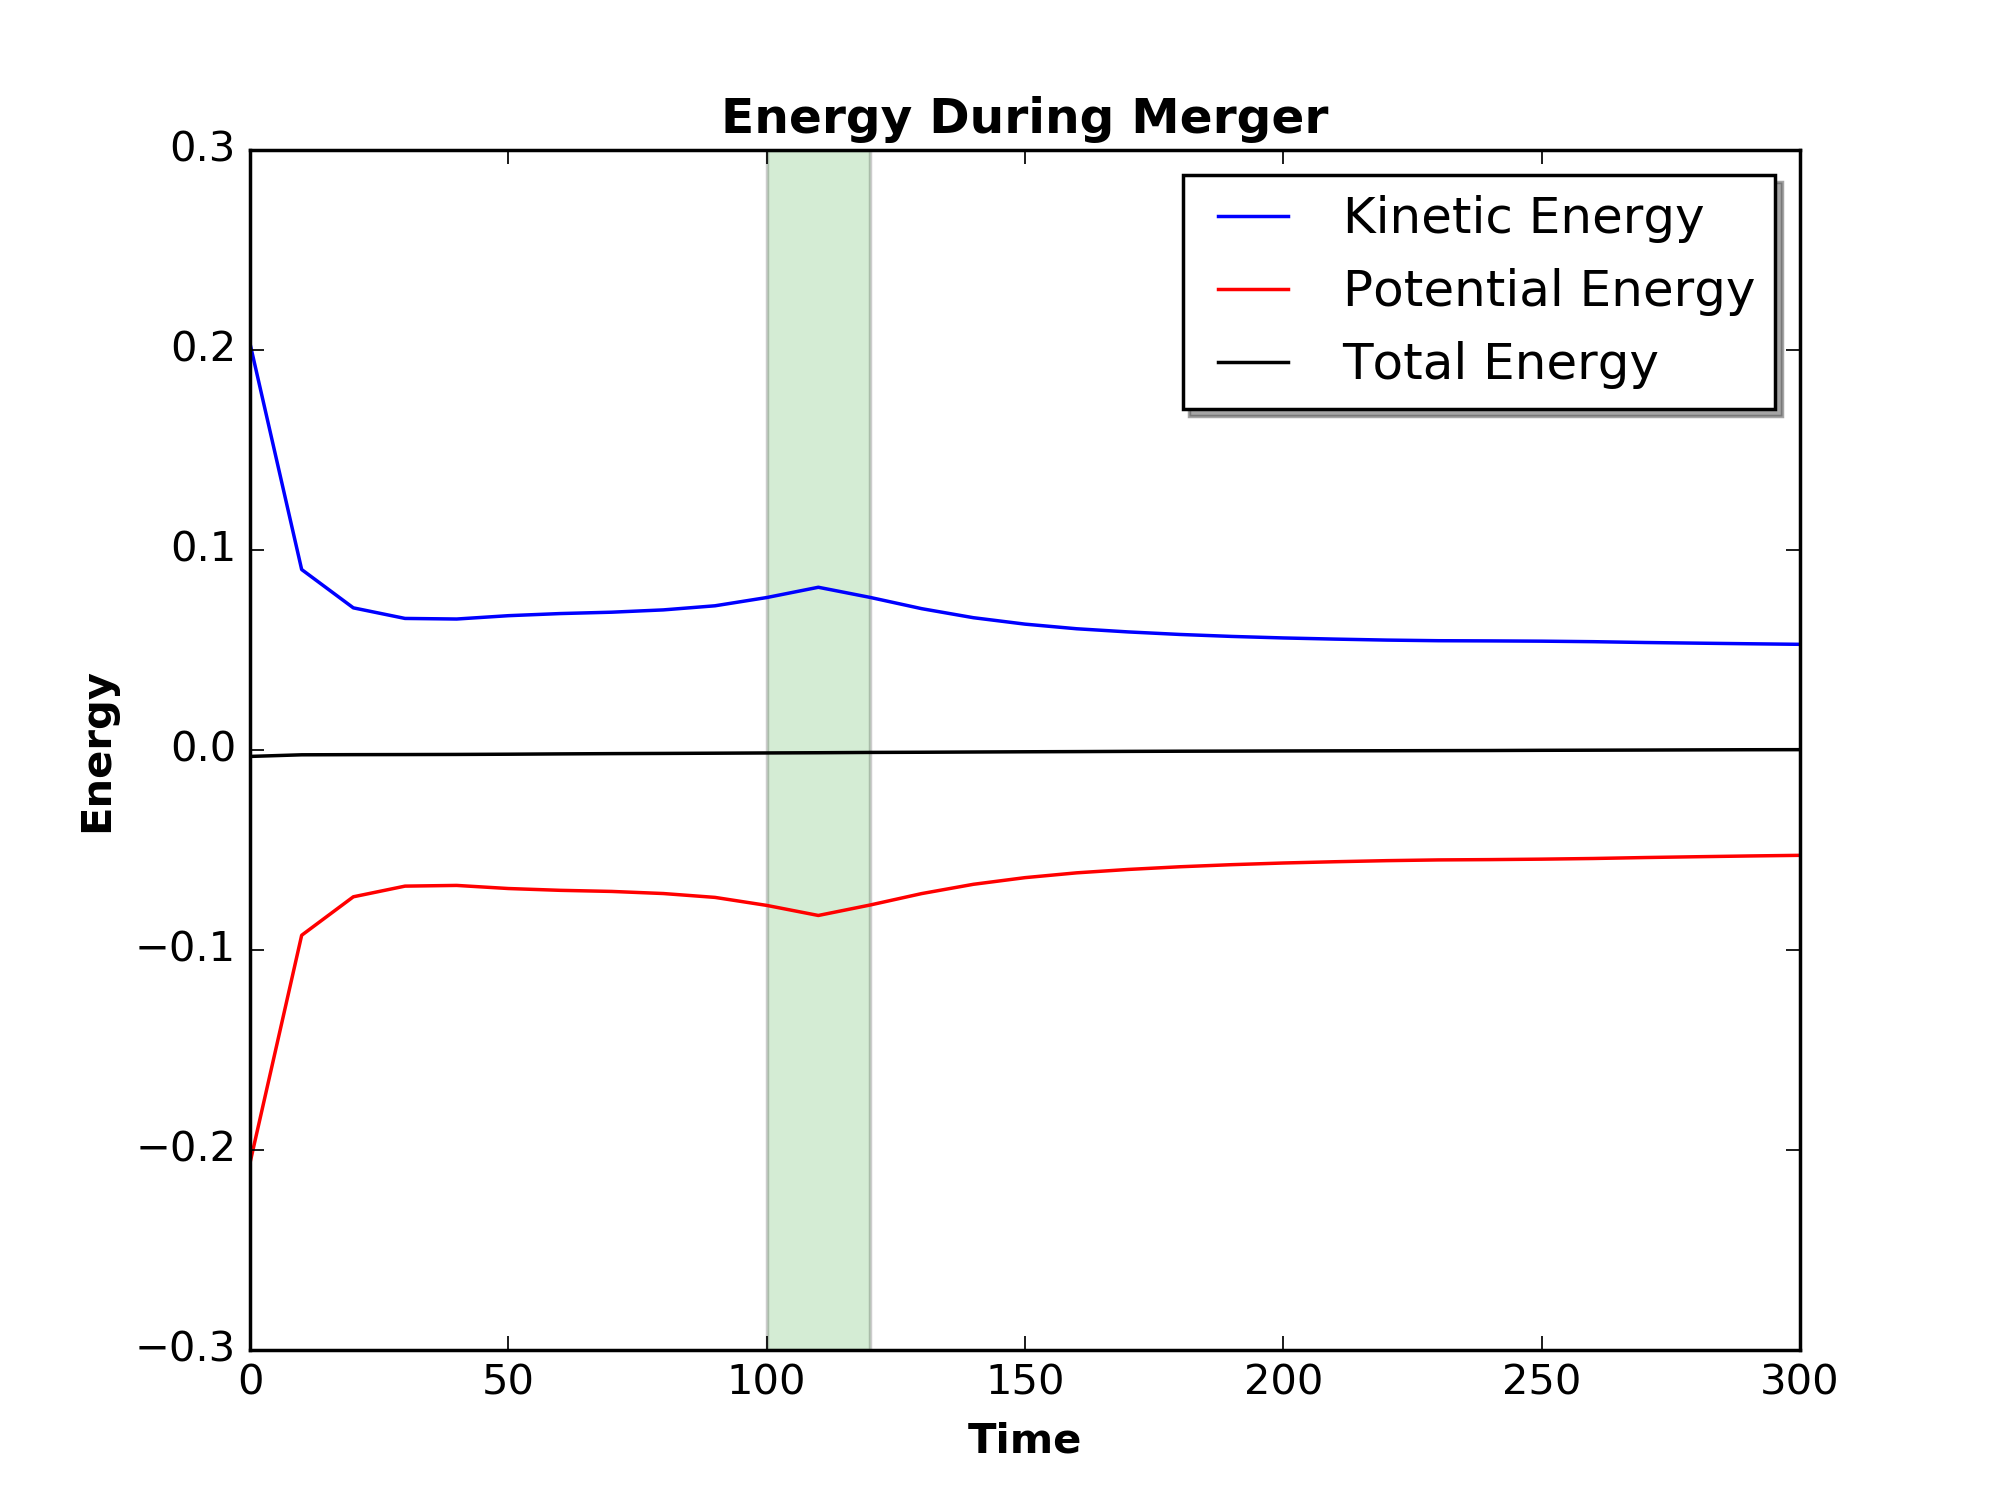
\includegraphics[width=\linewidth]{Energy_of_merger-model1.png}
        \caption[]%
        {{Kinetic energy, potential energy, and total energy versus time.}}
        
        \label{fig:totalenergy}
    \end{subfigure} %'
    \hfill
    \begin{subfigure}[b]{.475\textwidth}
        \centering
        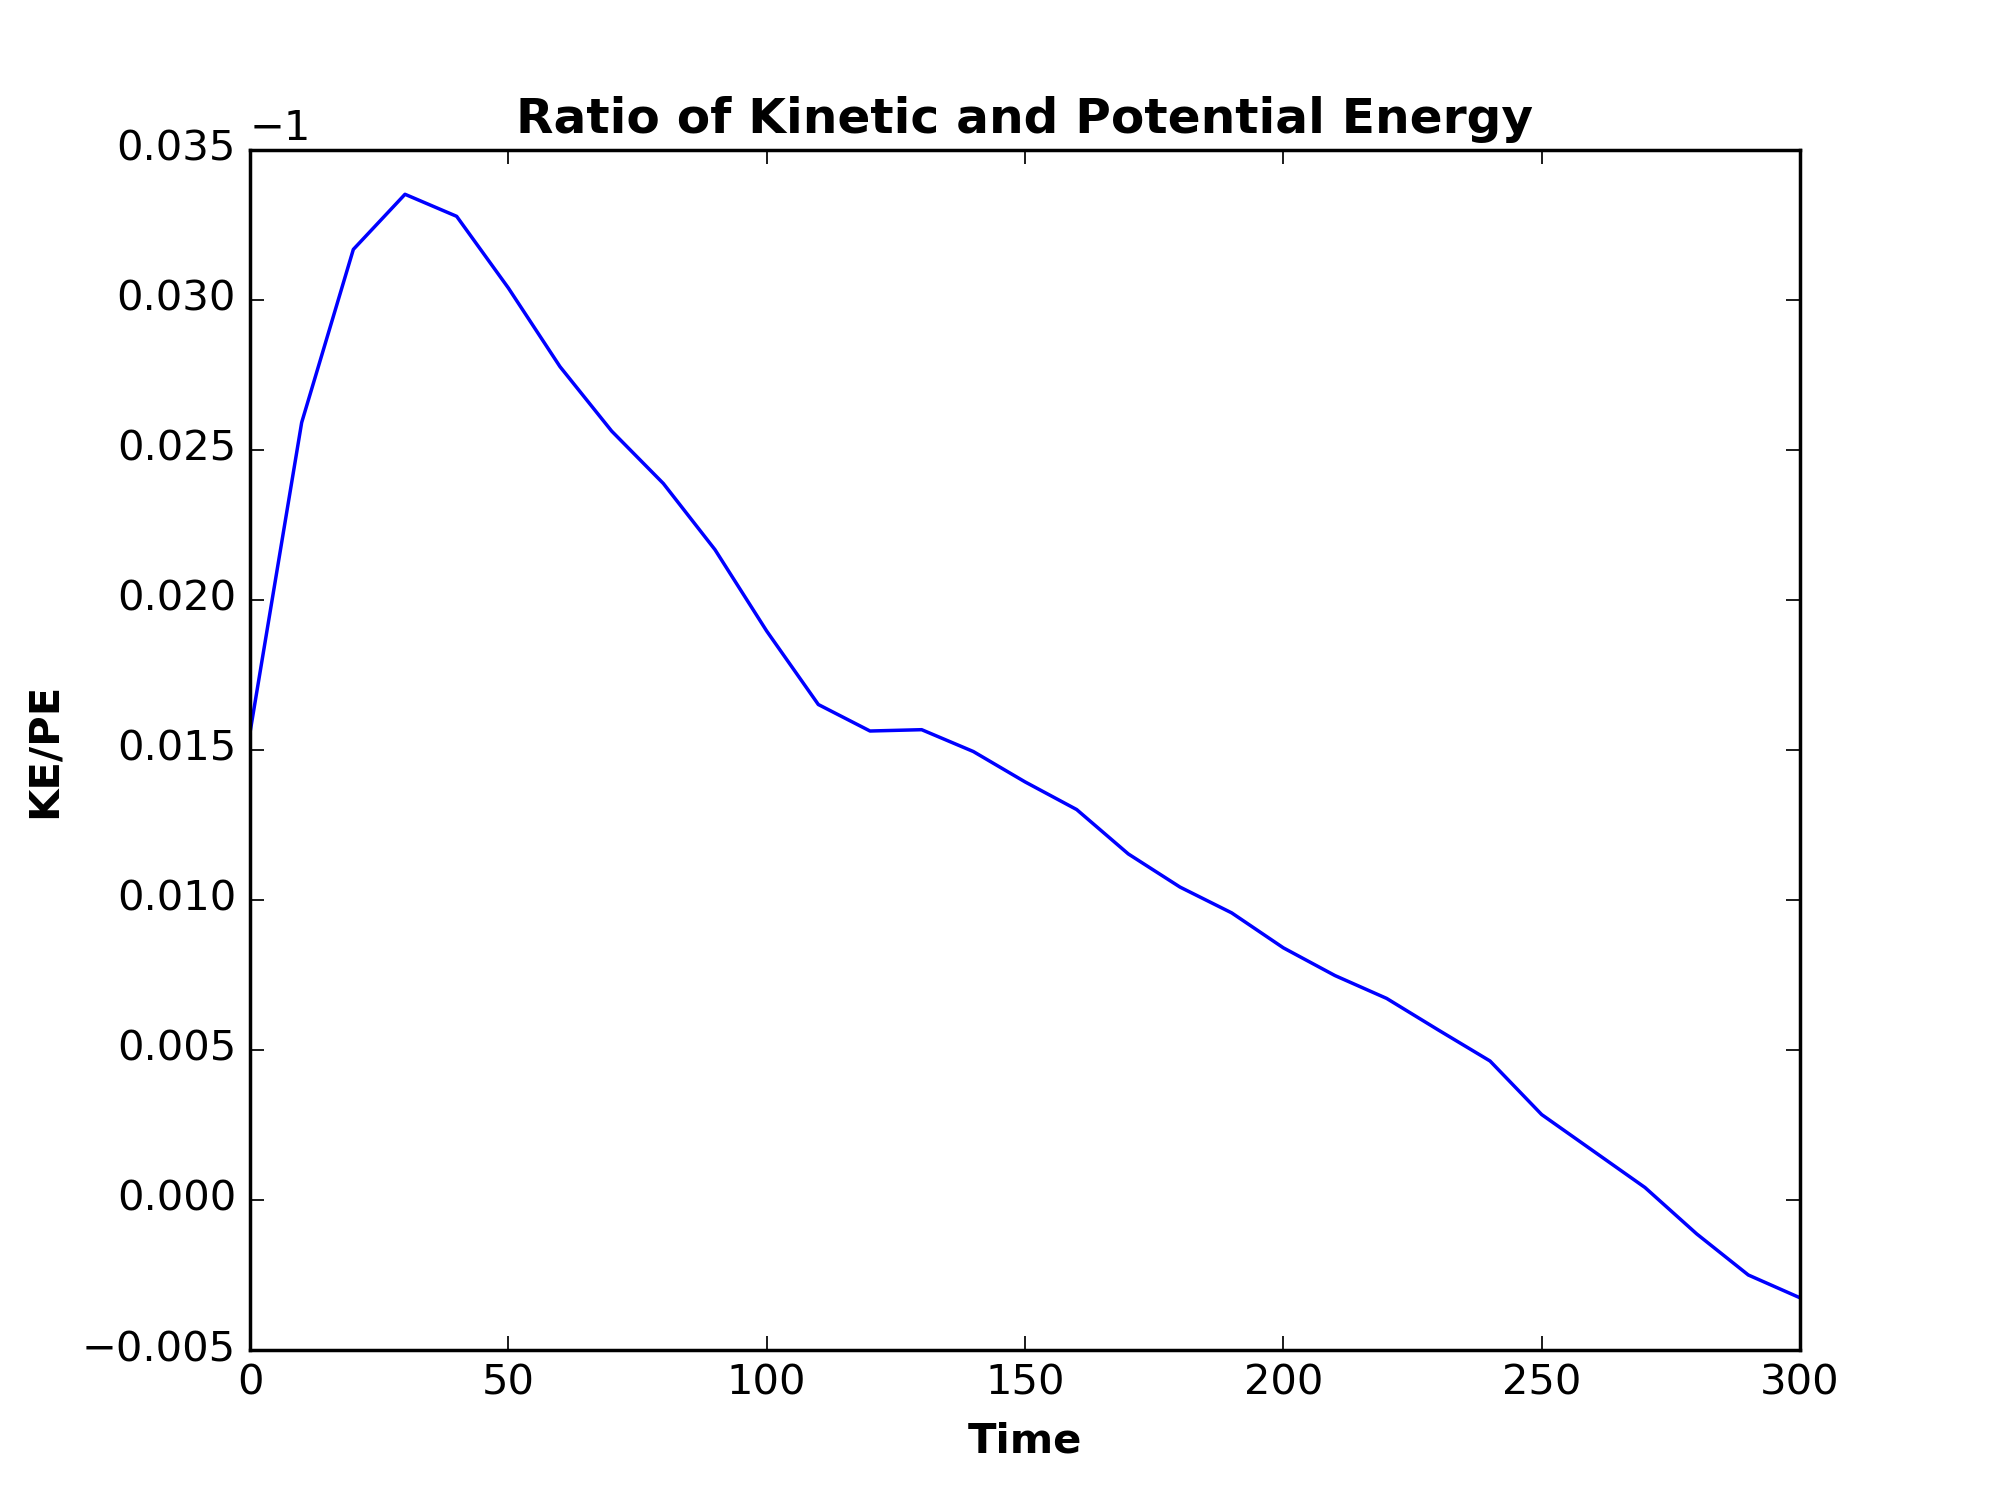
\includegraphics[width=\linewidth]{ratioofkineticandpotential_mod1.png}
        \caption[]%
        {{The ratio between kinetic and potential energy versus time.}}
        \label{fig:ratiomerger1}
    \end{subfigure} %
    \caption[]
        {The plots above illustrate the energy change during the merger highlighted in Figure~\ref{fig:merger1}. The green shaded area in Figure~\ref{fig:totalenergy} highlights a particular perturbation in the energy of the system corresponding to time step $110$ seen in Figure~\ref{fig:merger1_t110}.} 
        \label{fig:energyofmerger1}
\end{figure}

Something interesting to note is the slight perturbation (highlighted in green) seen in the curves of kinetic and potential energy in Figure~\ref{fig:totalenergy}. This area corresponds to the merger sequence of Figure~\ref{fig:merger1_t110}. This time stamp happens well after the initial start of the merger; thus, something is occurring at this time stamp that increases the kinetic energy of the system. Perhaps this is when the merger becomes complete.

\begin{figure}[H]
        \centering
        \begin{subfigure}[b]{0.48\textwidth}
            \centering
            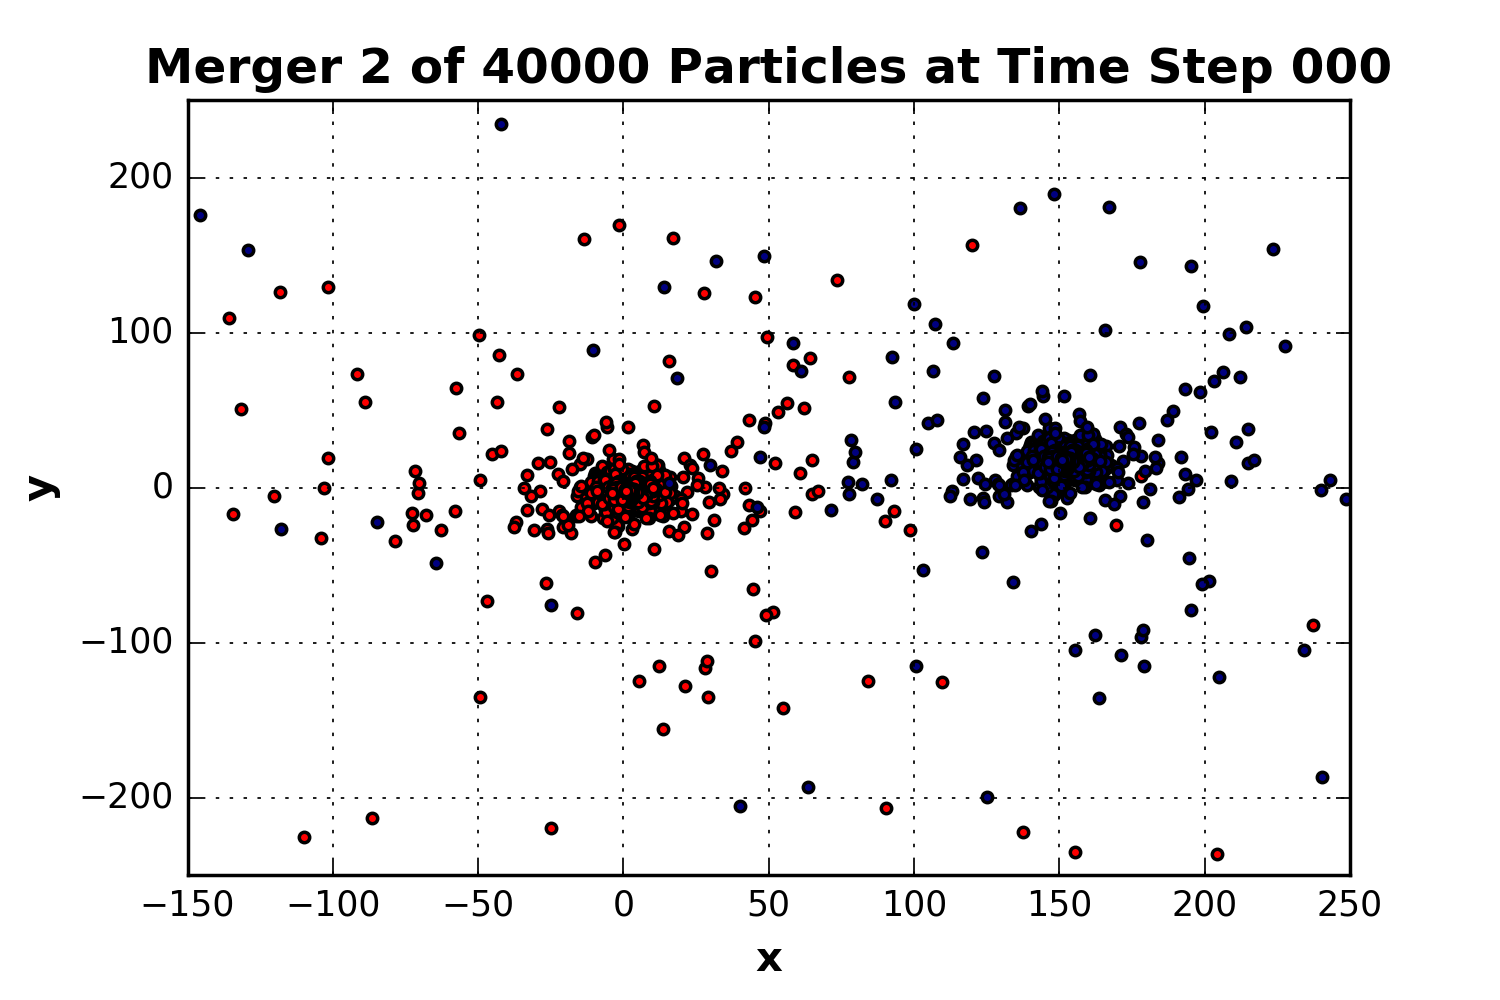
\includegraphics[width=\linewidth]{merger2t000.png}
            \caption[]%
            {{\small The two elliptical galaxies separated by an x-shift of $150$ and y-shift of $20$.}}    
            \label{fig:merger2_t00}
        \end{subfigure}
        \hfill
        \begin{subfigure}[b]{0.48\textwidth}  
            \centering 
            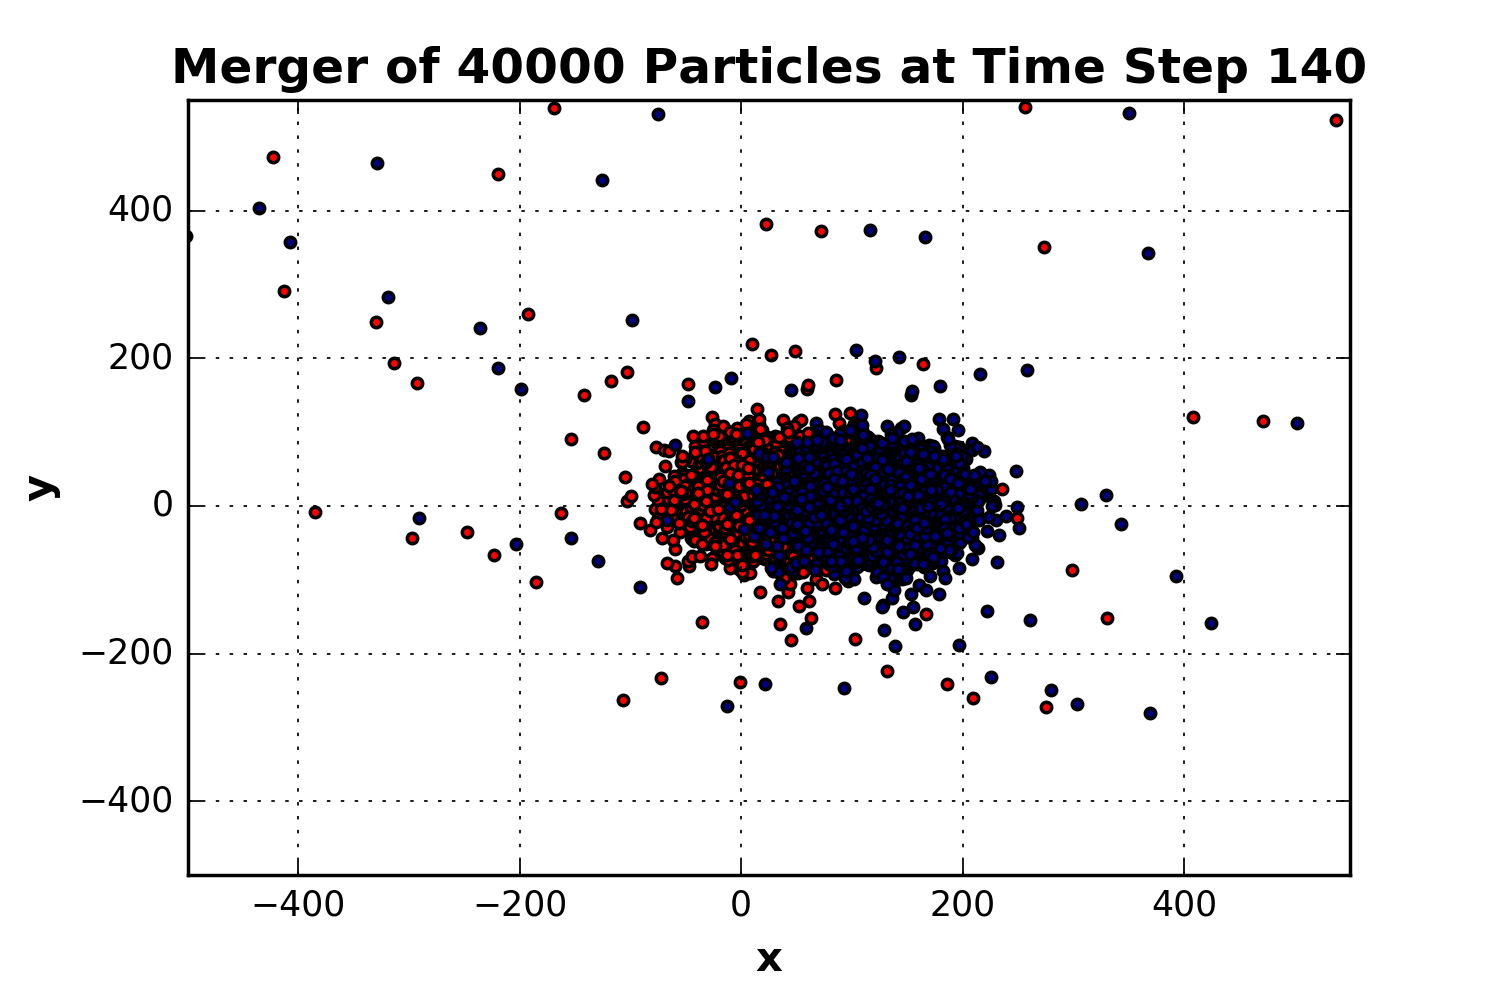
\includegraphics[width=\linewidth]{merger2_t140.png}
            \caption[]%
            {{\small The two elliptical galaxies merging at a time step of $140$.}}    
            \label{fig:merger2_t140}
        \end{subfigure}
        \vskip\baselineskip
        \begin{subfigure}[b]{0.48\textwidth}   
            \centering 
            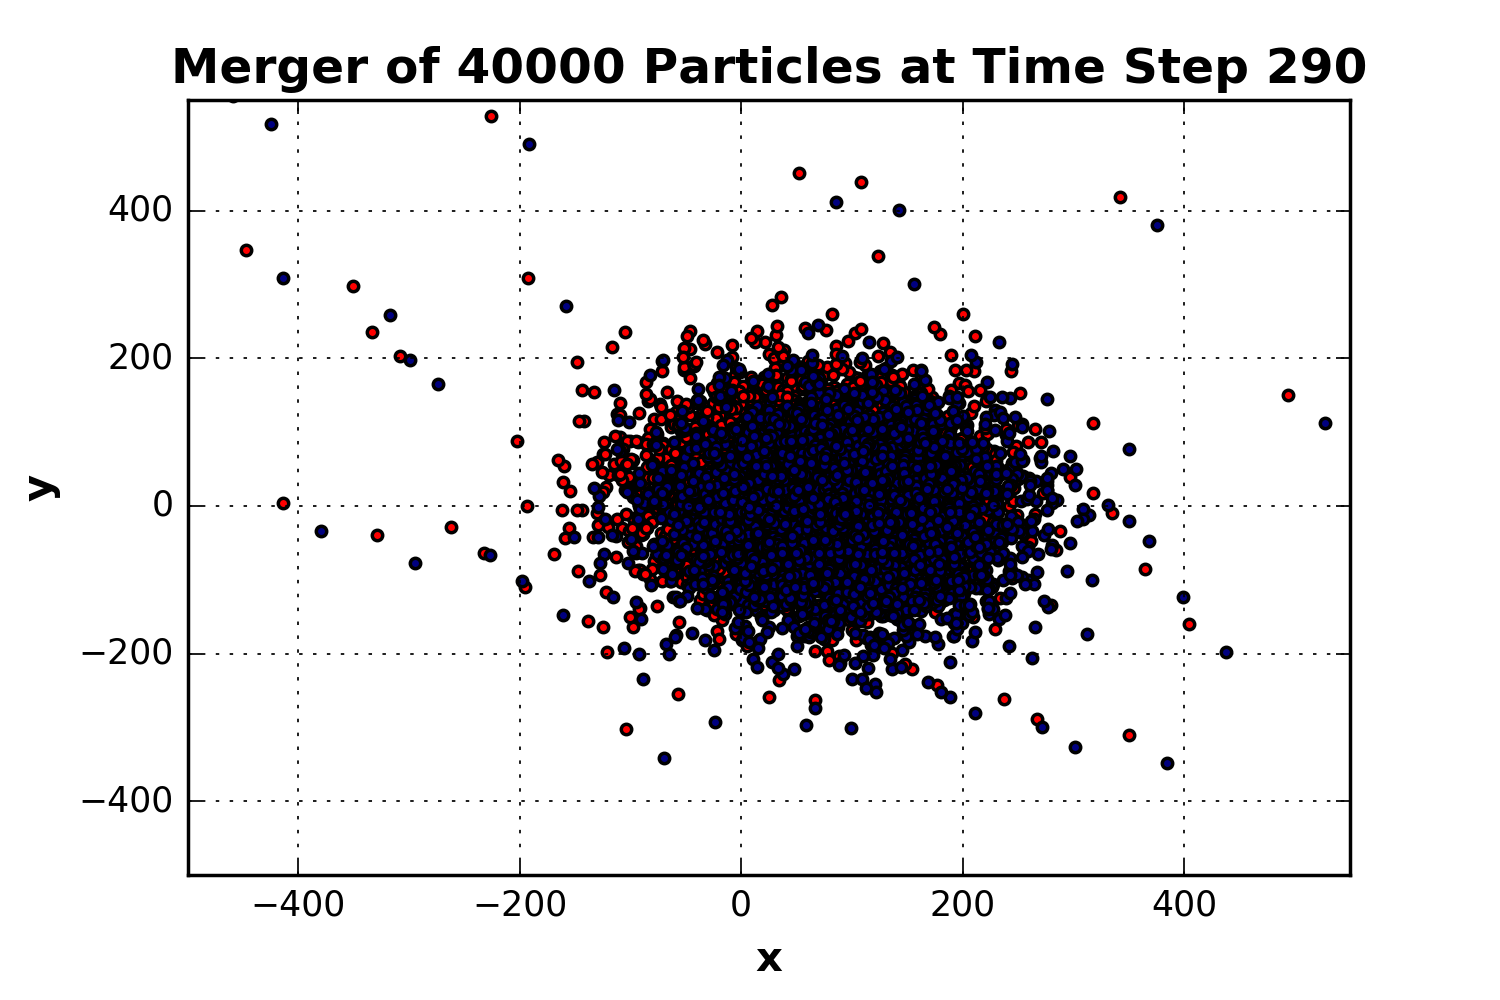
\includegraphics[width=\linewidth]{merger2_t290.png}
            \caption[]%
            {{\small The two elliptical galaxies completely merged at a time step of $290$.}}    
            \label{fig:merger2_t200}
        \end{subfigure}
        \quad
        \begin{subfigure}[b]{0.48\textwidth}   
            \centering 
            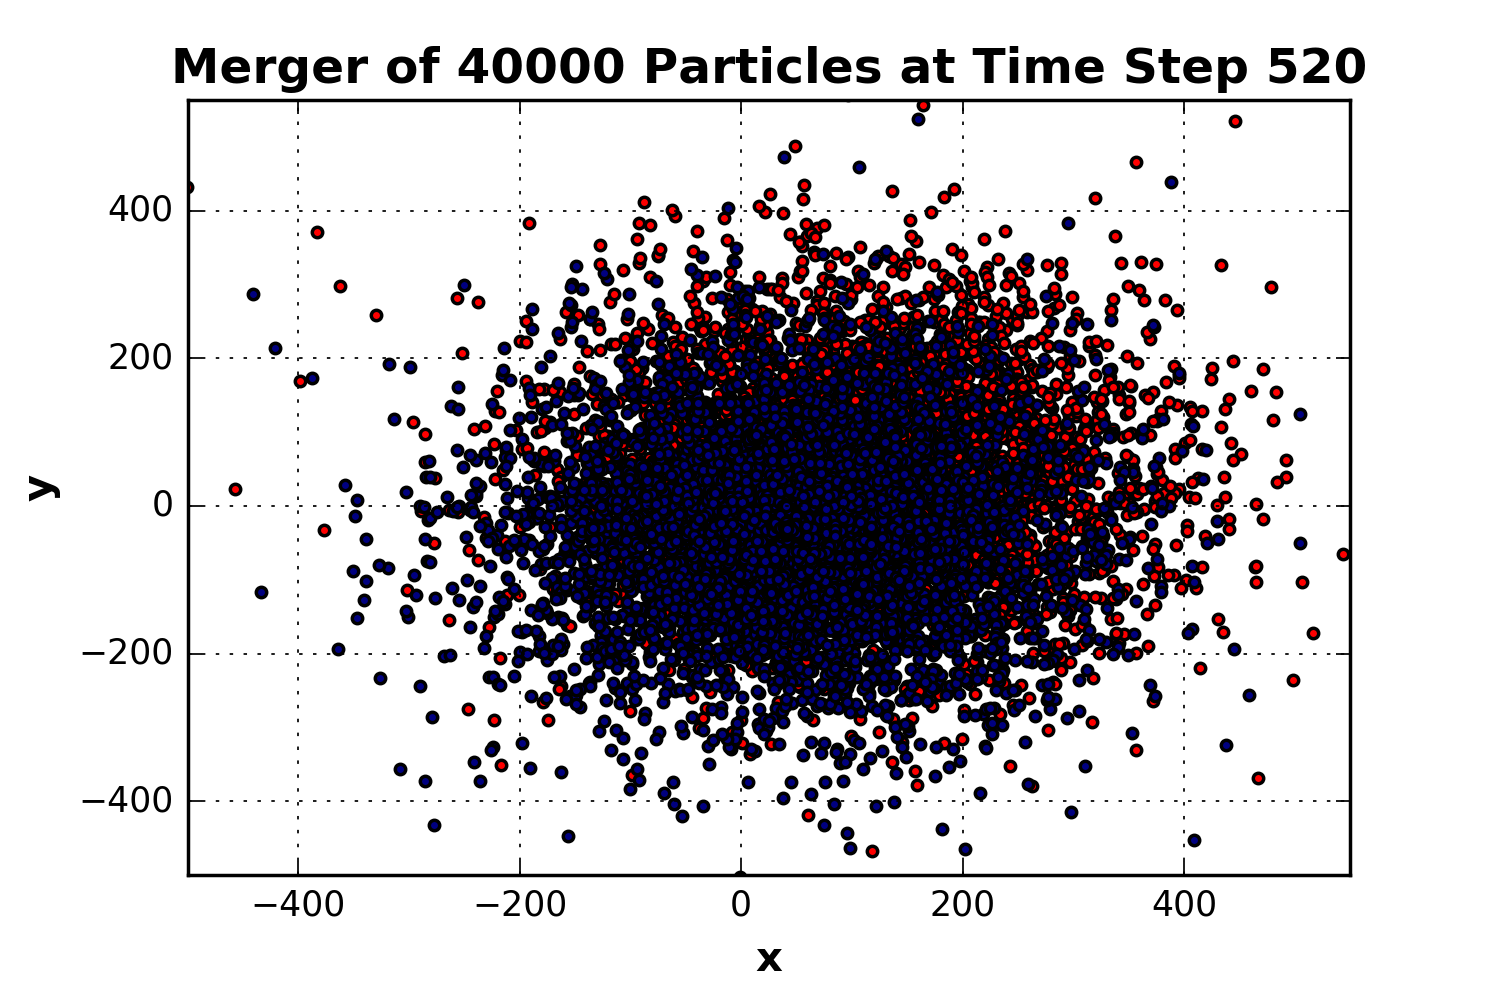
\includegraphics[width=\textwidth]{merger2_t520.png}\
            \caption[]%
            {{\small The two elliptical galaxies after the merger at a time step of $520$}}
            \label{fig:merger2_t520}
        \end{subfigure}
        \caption[]
        {The plots above illustrate the second merger of two clouds of $20000$ particles each at different time steps.}
        \label{fig:merger2}
    \end{figure}
    
\begin{figure}[H]
\centering 
    \begin{subfigure}[b]{.475\textwidth}
        \centering
        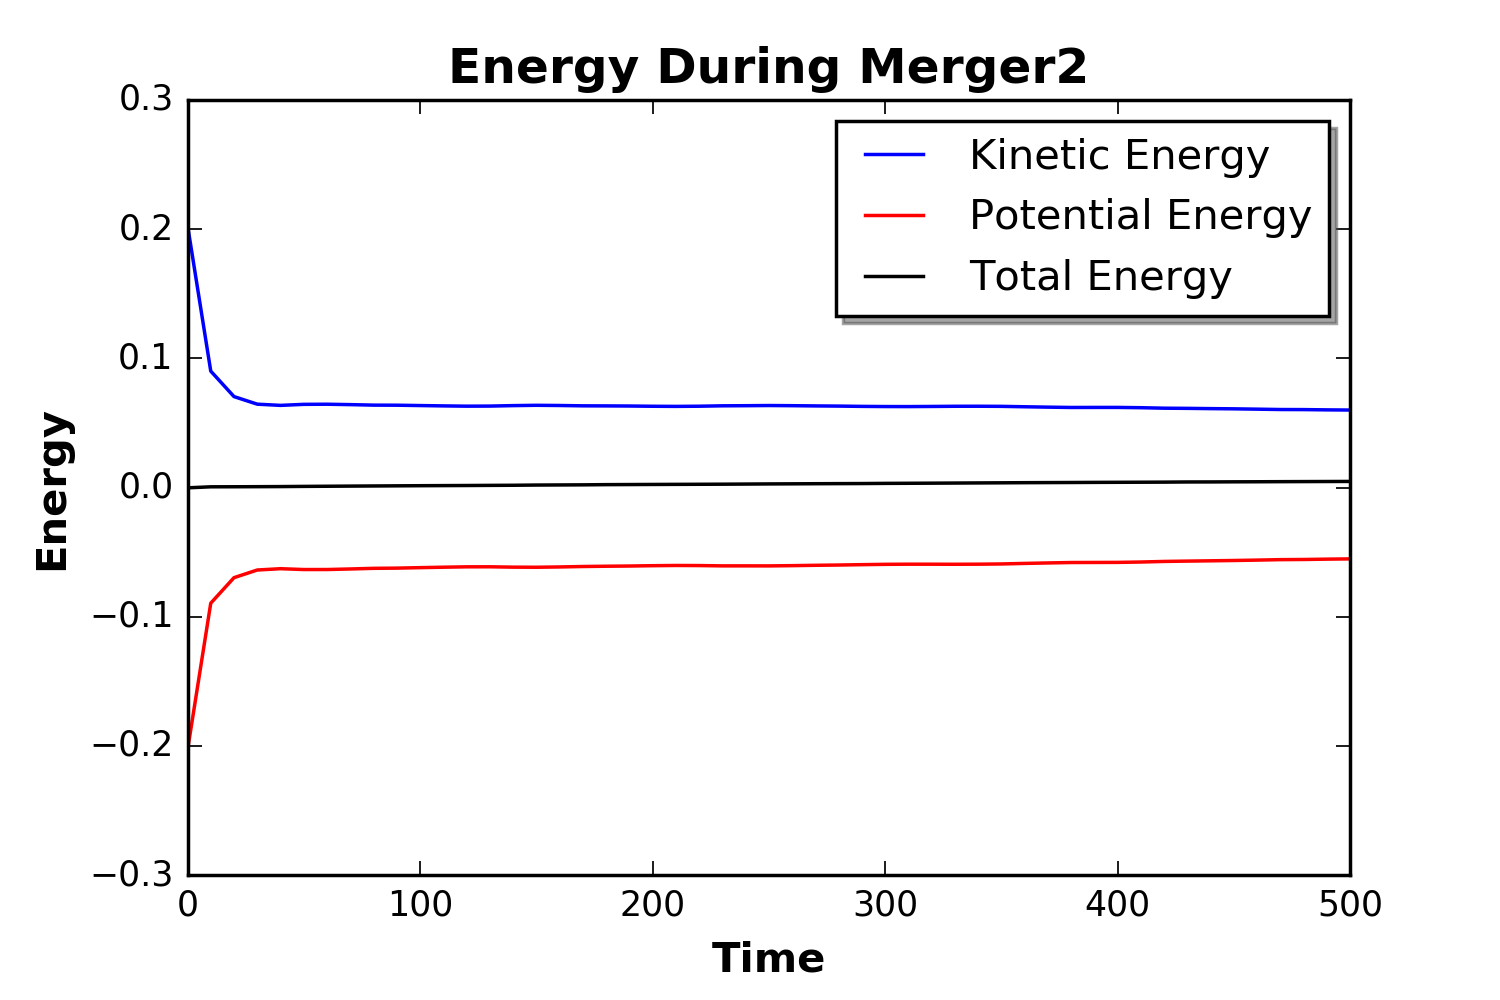
\includegraphics[width=\linewidth]{totenergy_merger2.png}
        \caption[]%
        {{Kinetic energy, potential energy, and total energy versus time.}}
    
        \label{fig:totalenergy_merger2}
    \end{subfigure} %'
    \hfill
    \begin{subfigure}[b]{.475\textwidth}
        \centering
        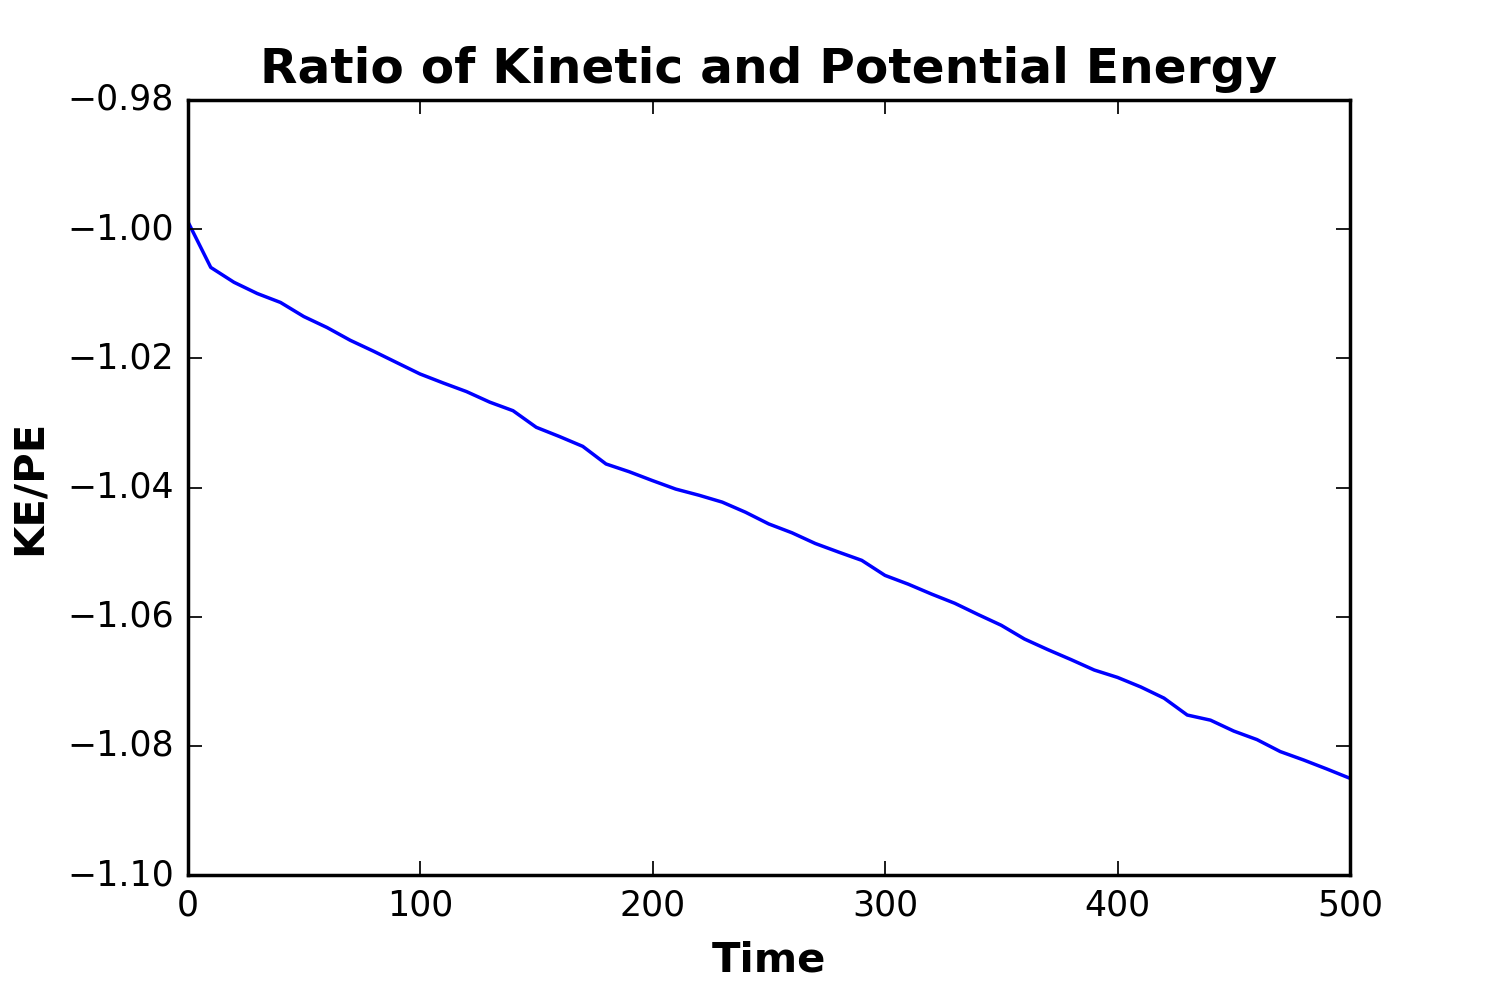
\includegraphics[width=\linewidth]{ratioenergy_merger2.png}
        \caption[]%
        {{The ratio between kinetic and potential energy versus time.}}
        \label{fig:ratiomerger2}
    \end{subfigure} %
    \caption[]
        {The plots above illustrate the energy change during the merger highlighted in Figure.} 
        \label{fig:energyofmerger2}
\end{figure}


\begin{figure}[!htb]
\minipage{0.32\textwidth}
  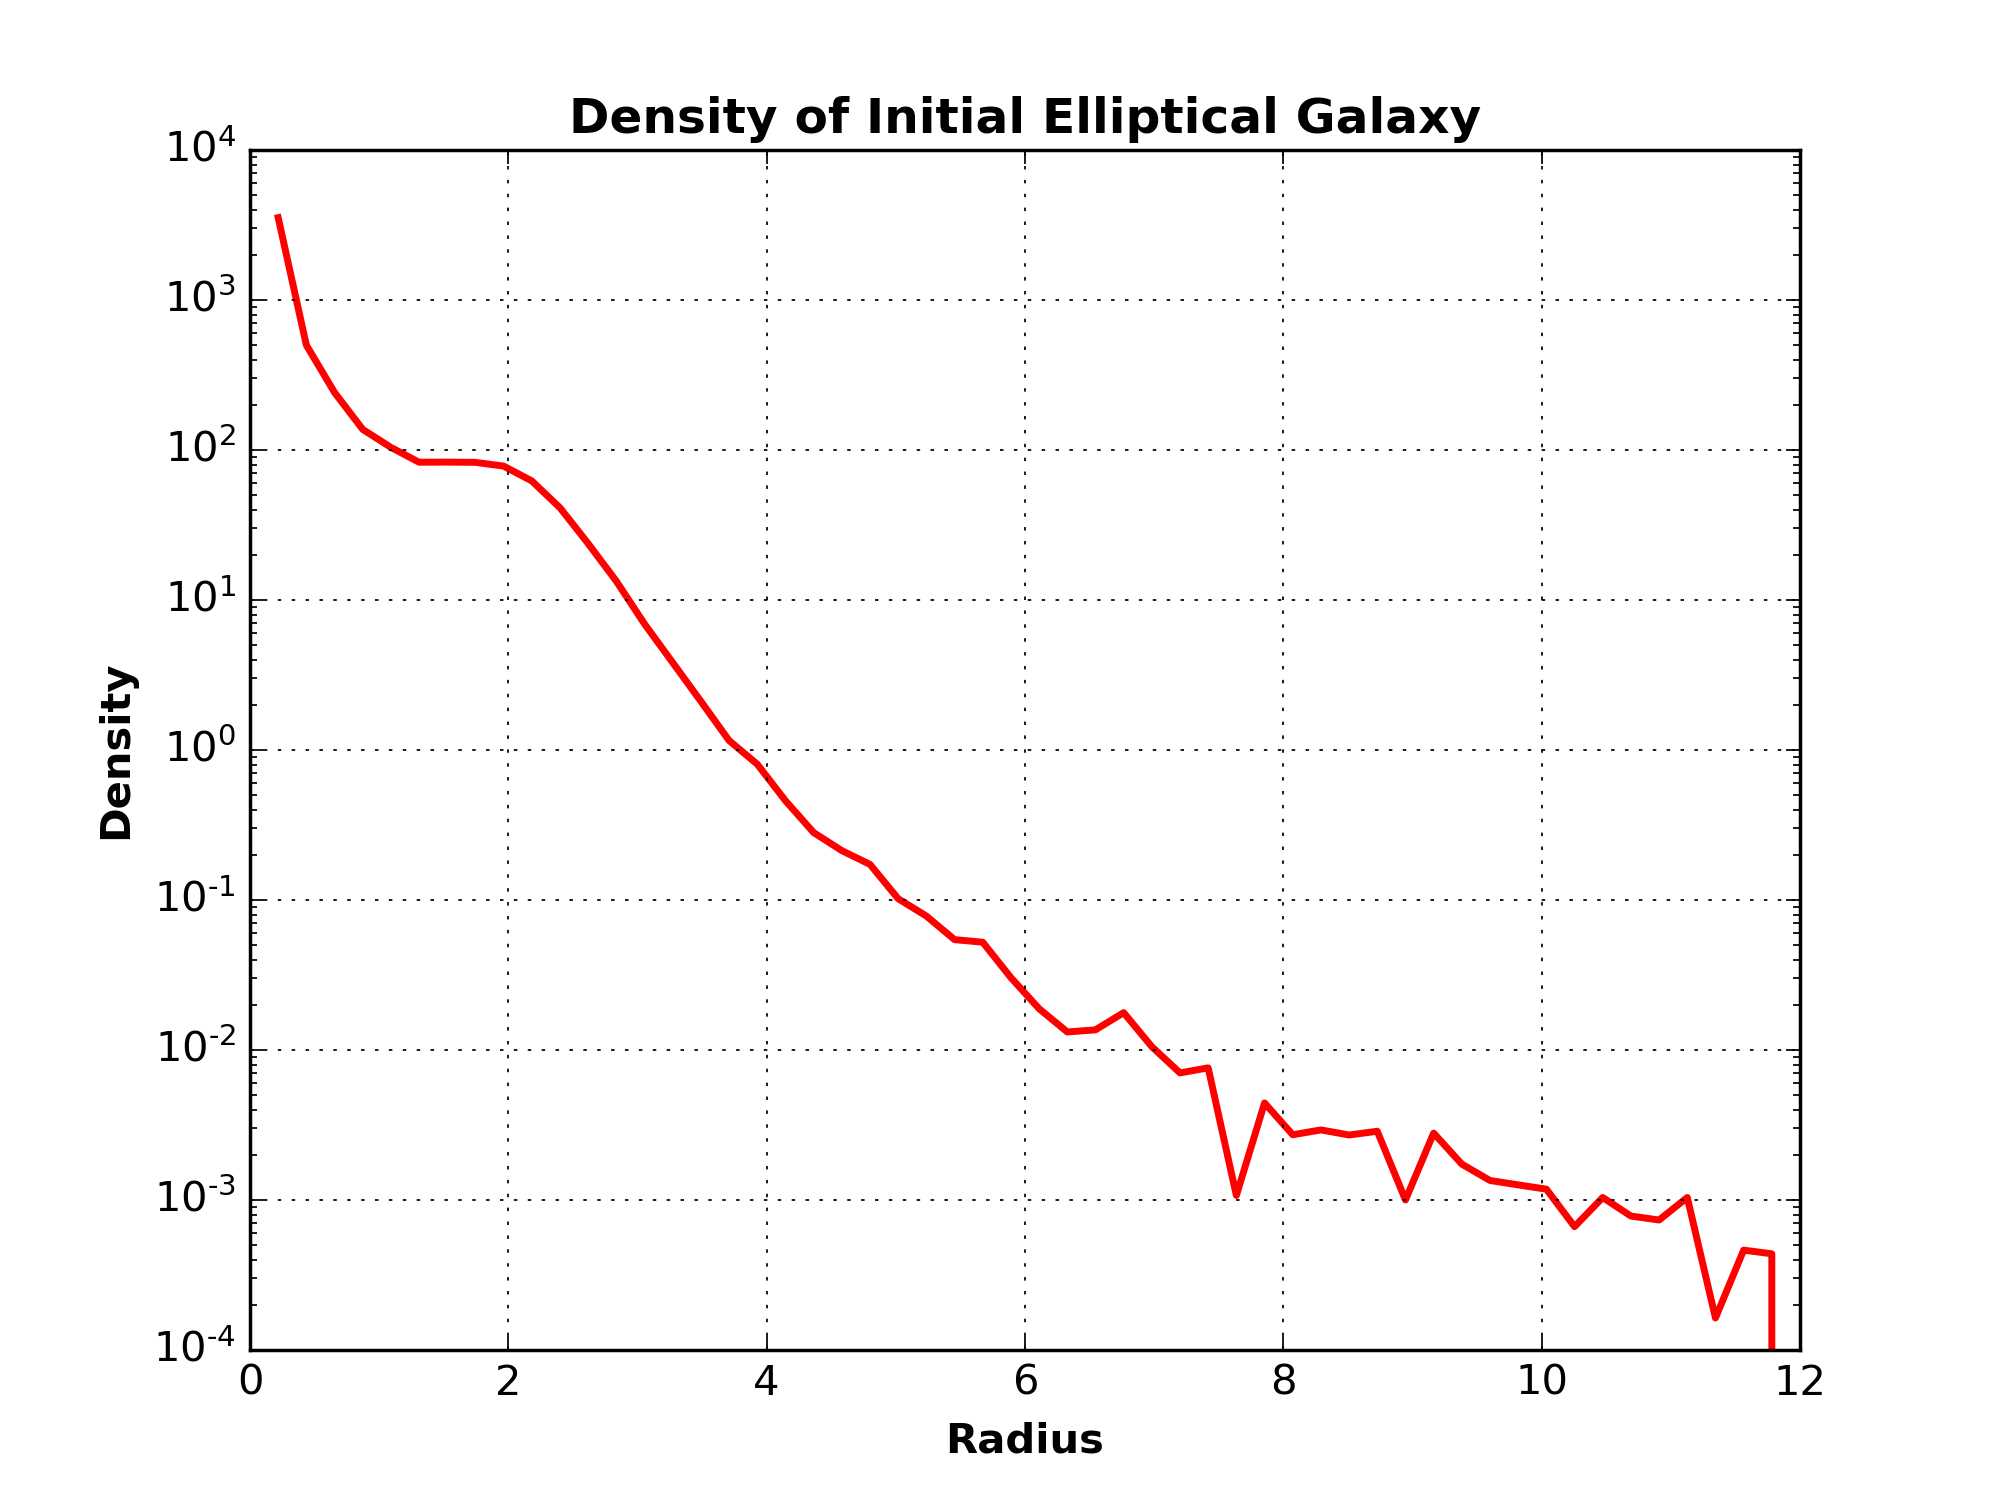
\includegraphics[width=\linewidth]{initial_density.png}
  \caption{The initial density.}
  \label{fig:density_initial}
\endminipage\hfill
\minipage{0.32\textwidth}
  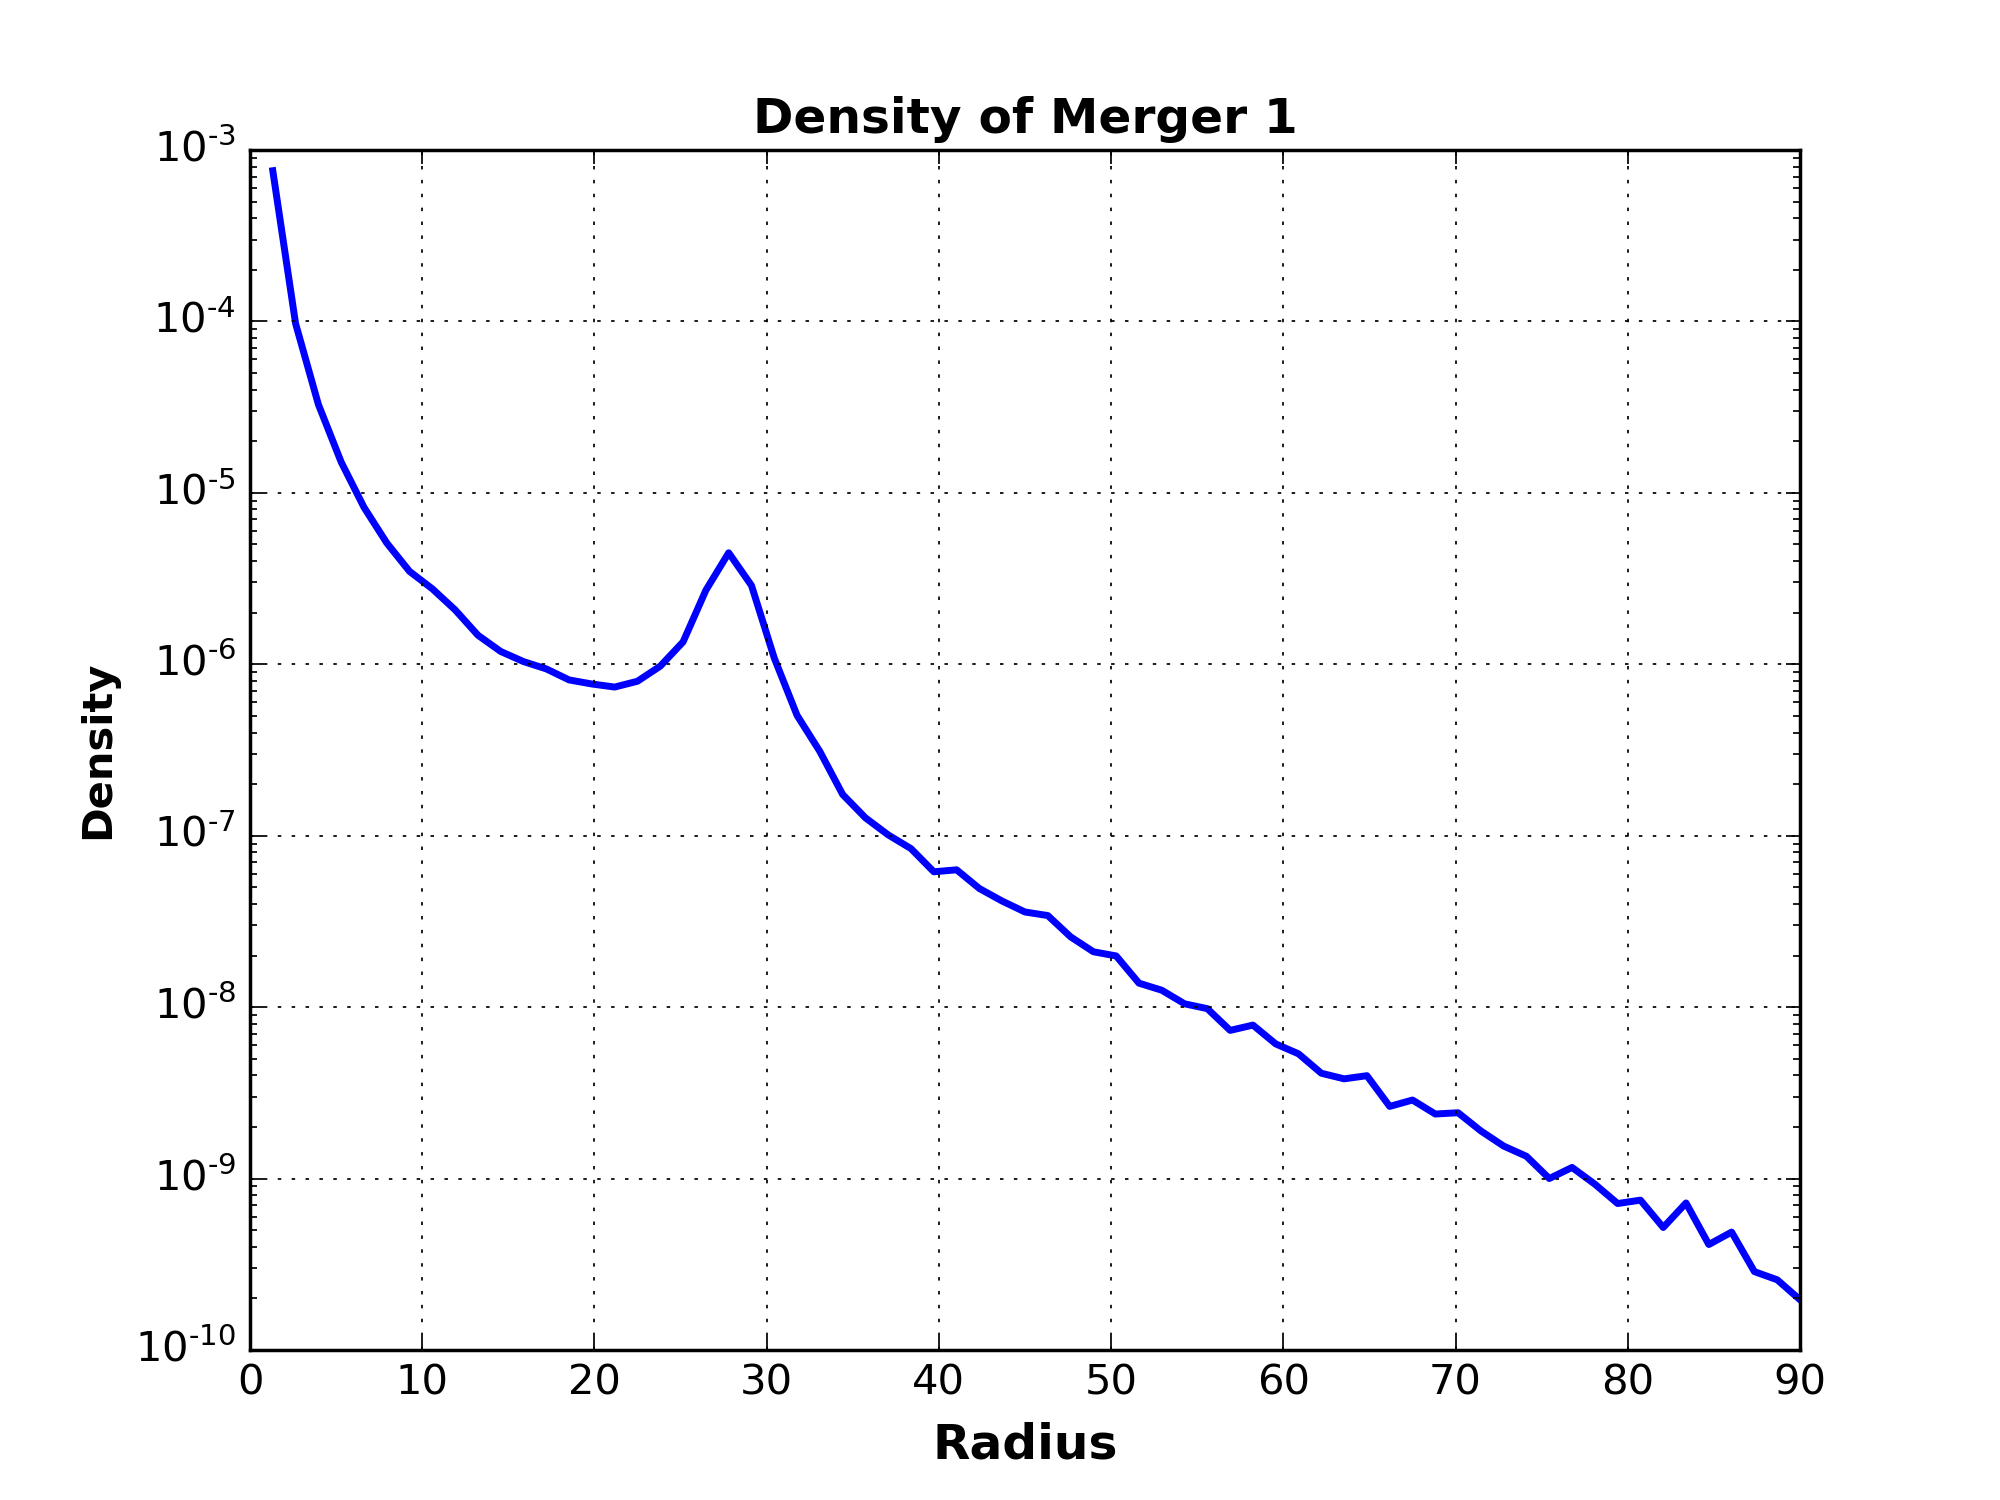
\includegraphics[width=\linewidth]{density_merger1.png}
  \caption{The density of the system after merger 1.}\label{fig:density_merger1}
\endminipage\hfill
\minipage{0.32\textwidth}
  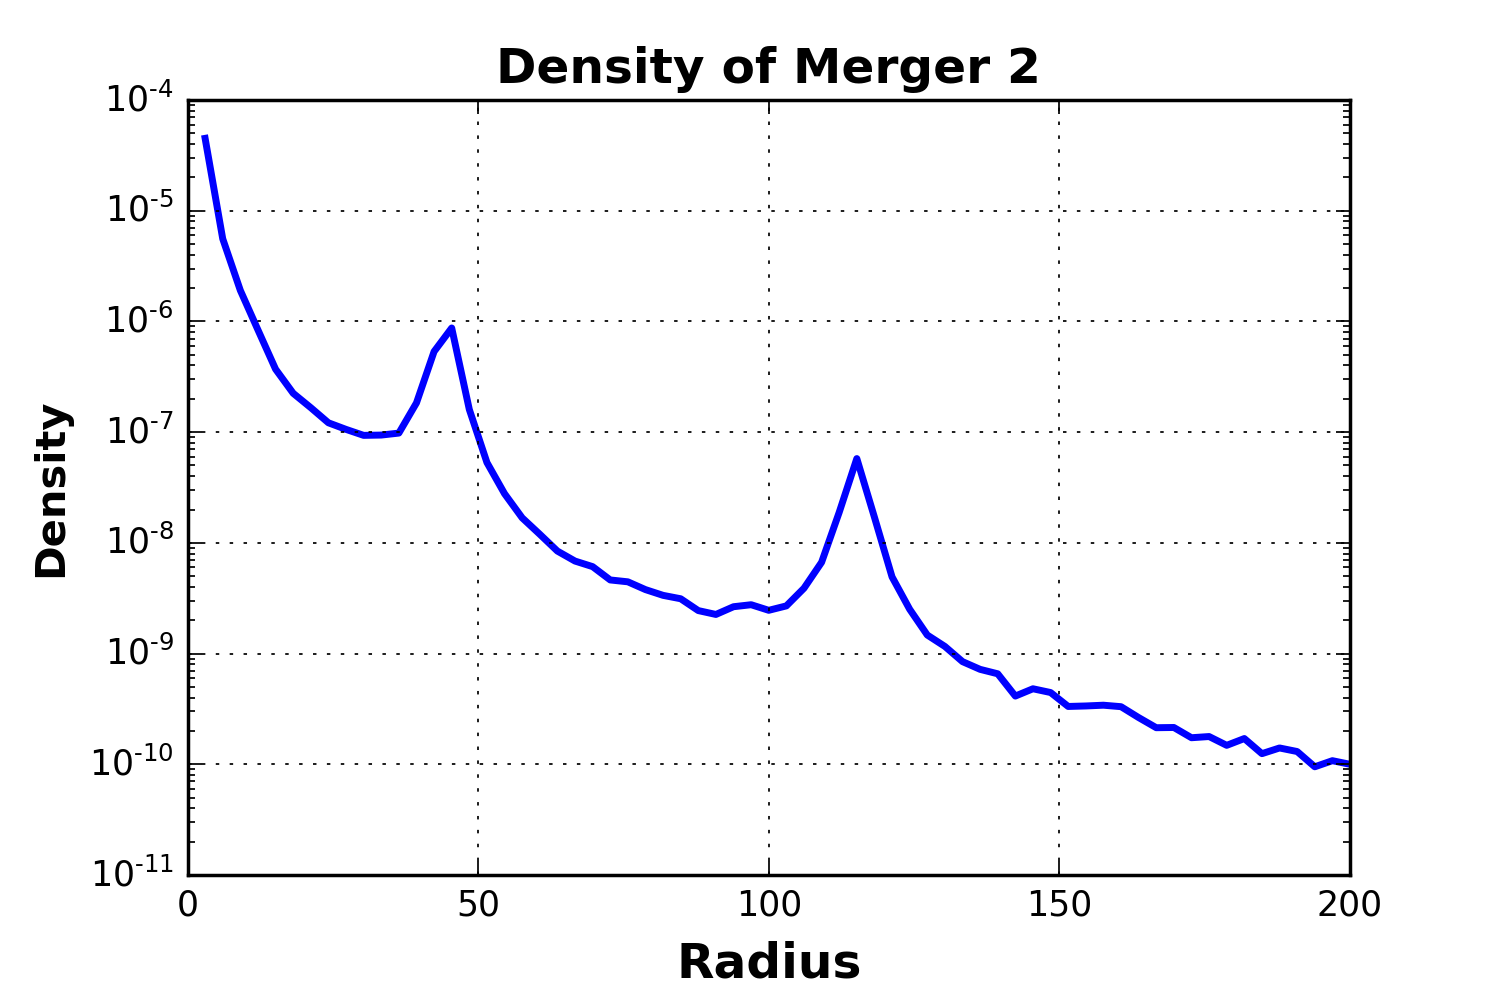
\includegraphics[width=\linewidth]{density_merger2.png}
  \caption{The density of the system after merger 2.}
  \label{fig:density_merger2}
\endminipage\hfill

\label{fig:density_of_systems}

\end{figure}


\begin{figure}[H]
\centering 
    \begin{subfigure}[b]{.475\textwidth}
        \centering
        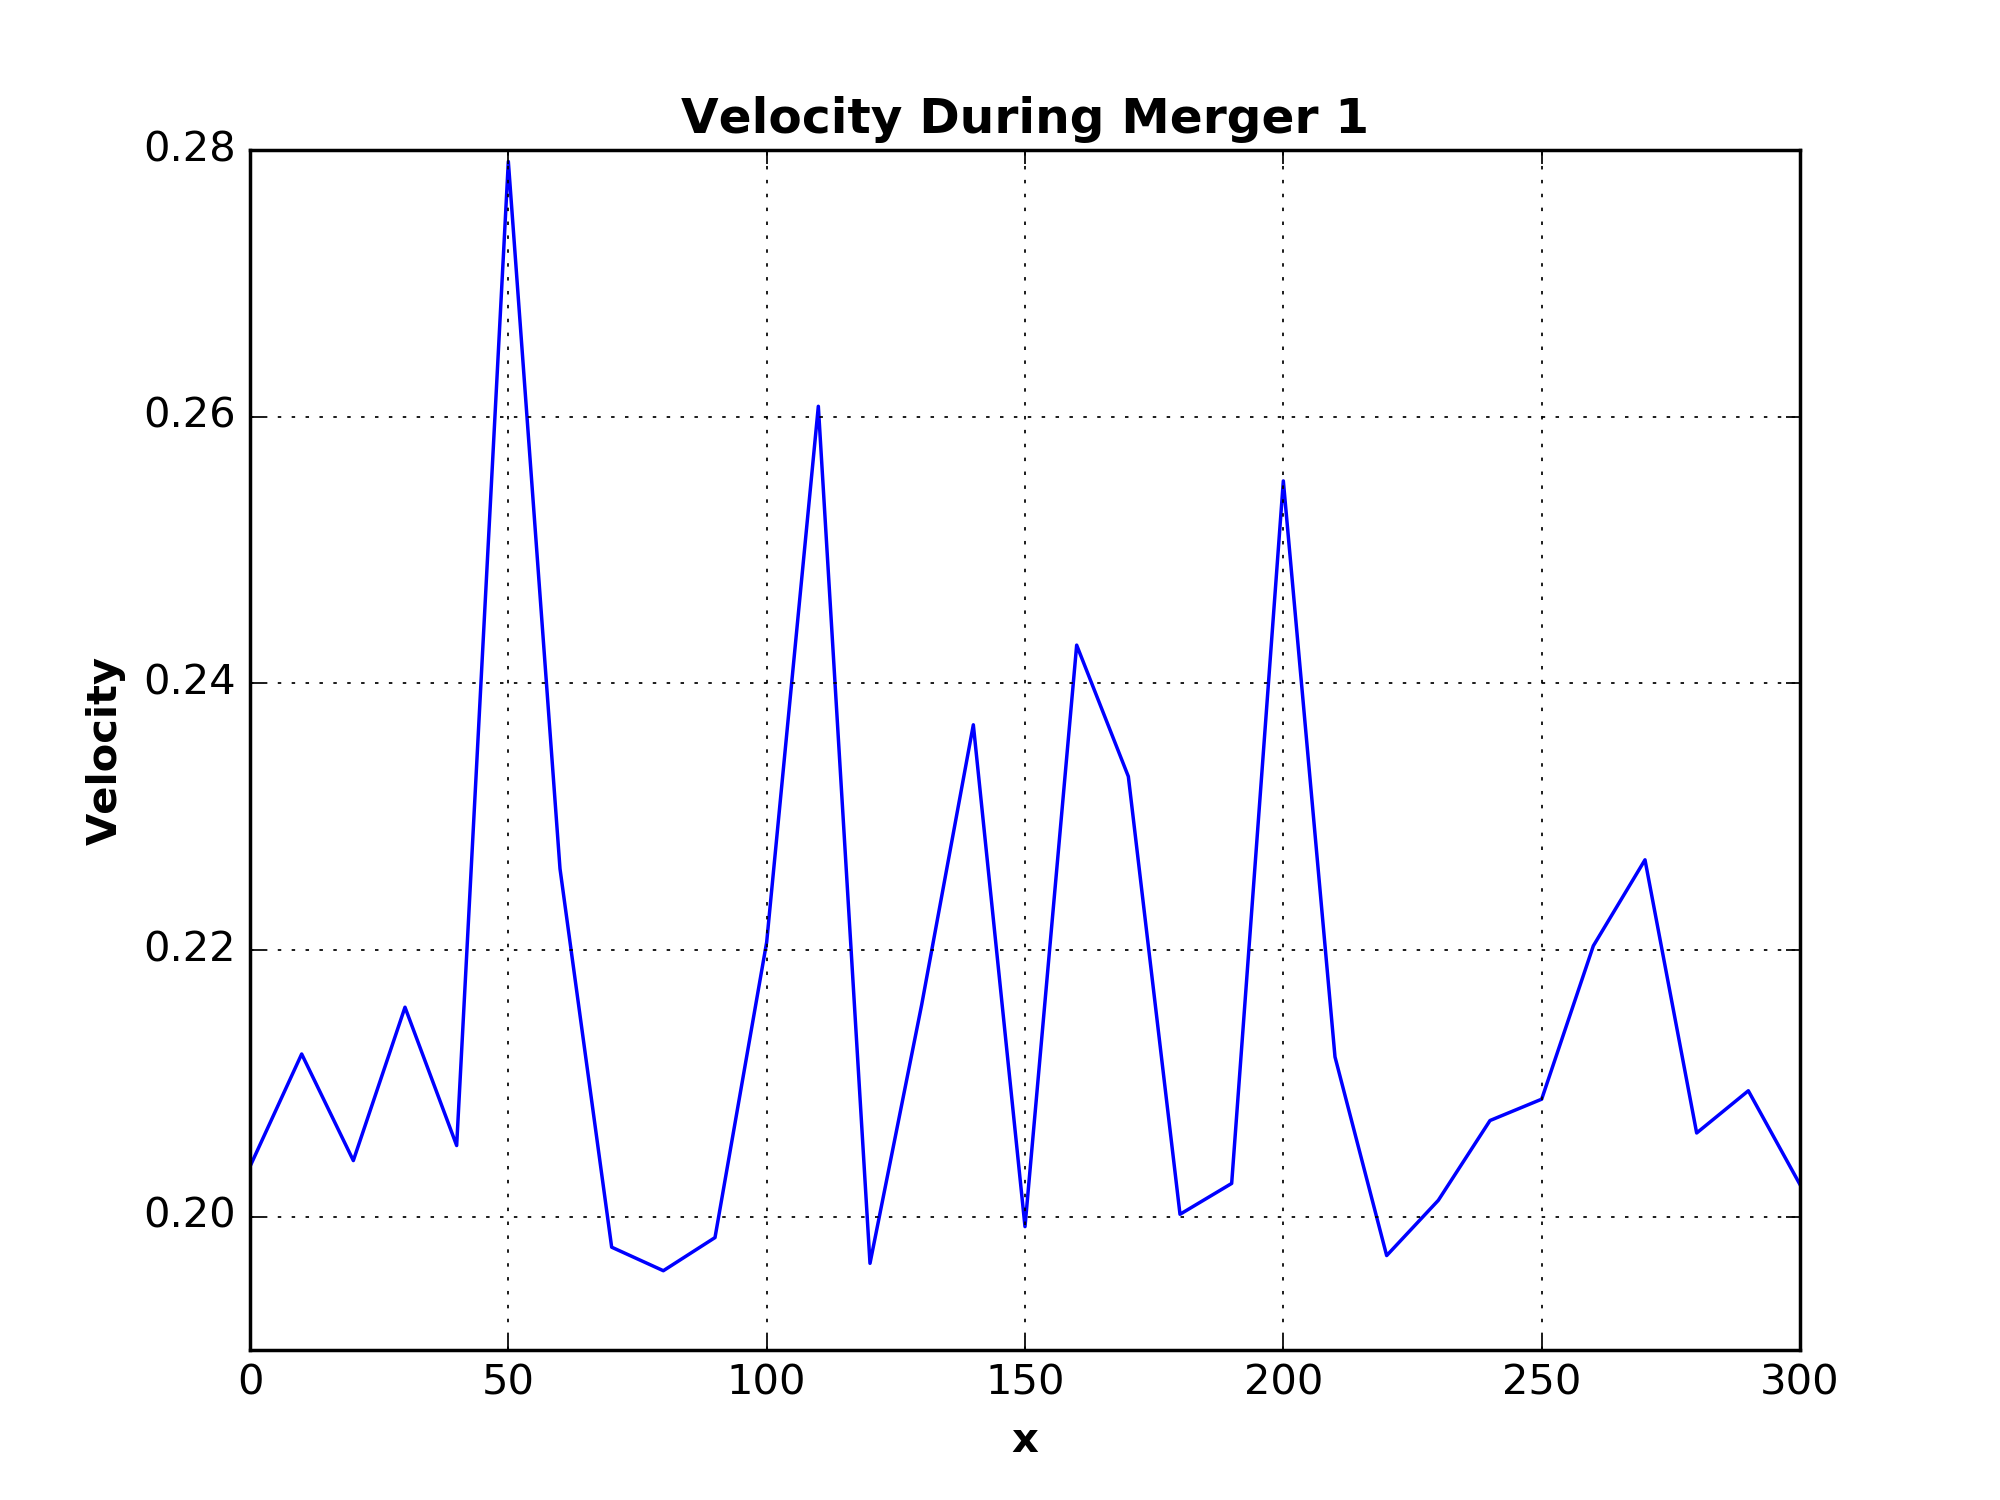
\includegraphics[width=\linewidth]{velocity_merger1.png}
        \caption[]%
        {{The velocity of the x-position during the first merger.}}
    
        \label{fig:velcoity_merger1}
    \end{subfigure} %'
    \hfill
    \begin{subfigure}[b]{.475\textwidth}
        \centering
        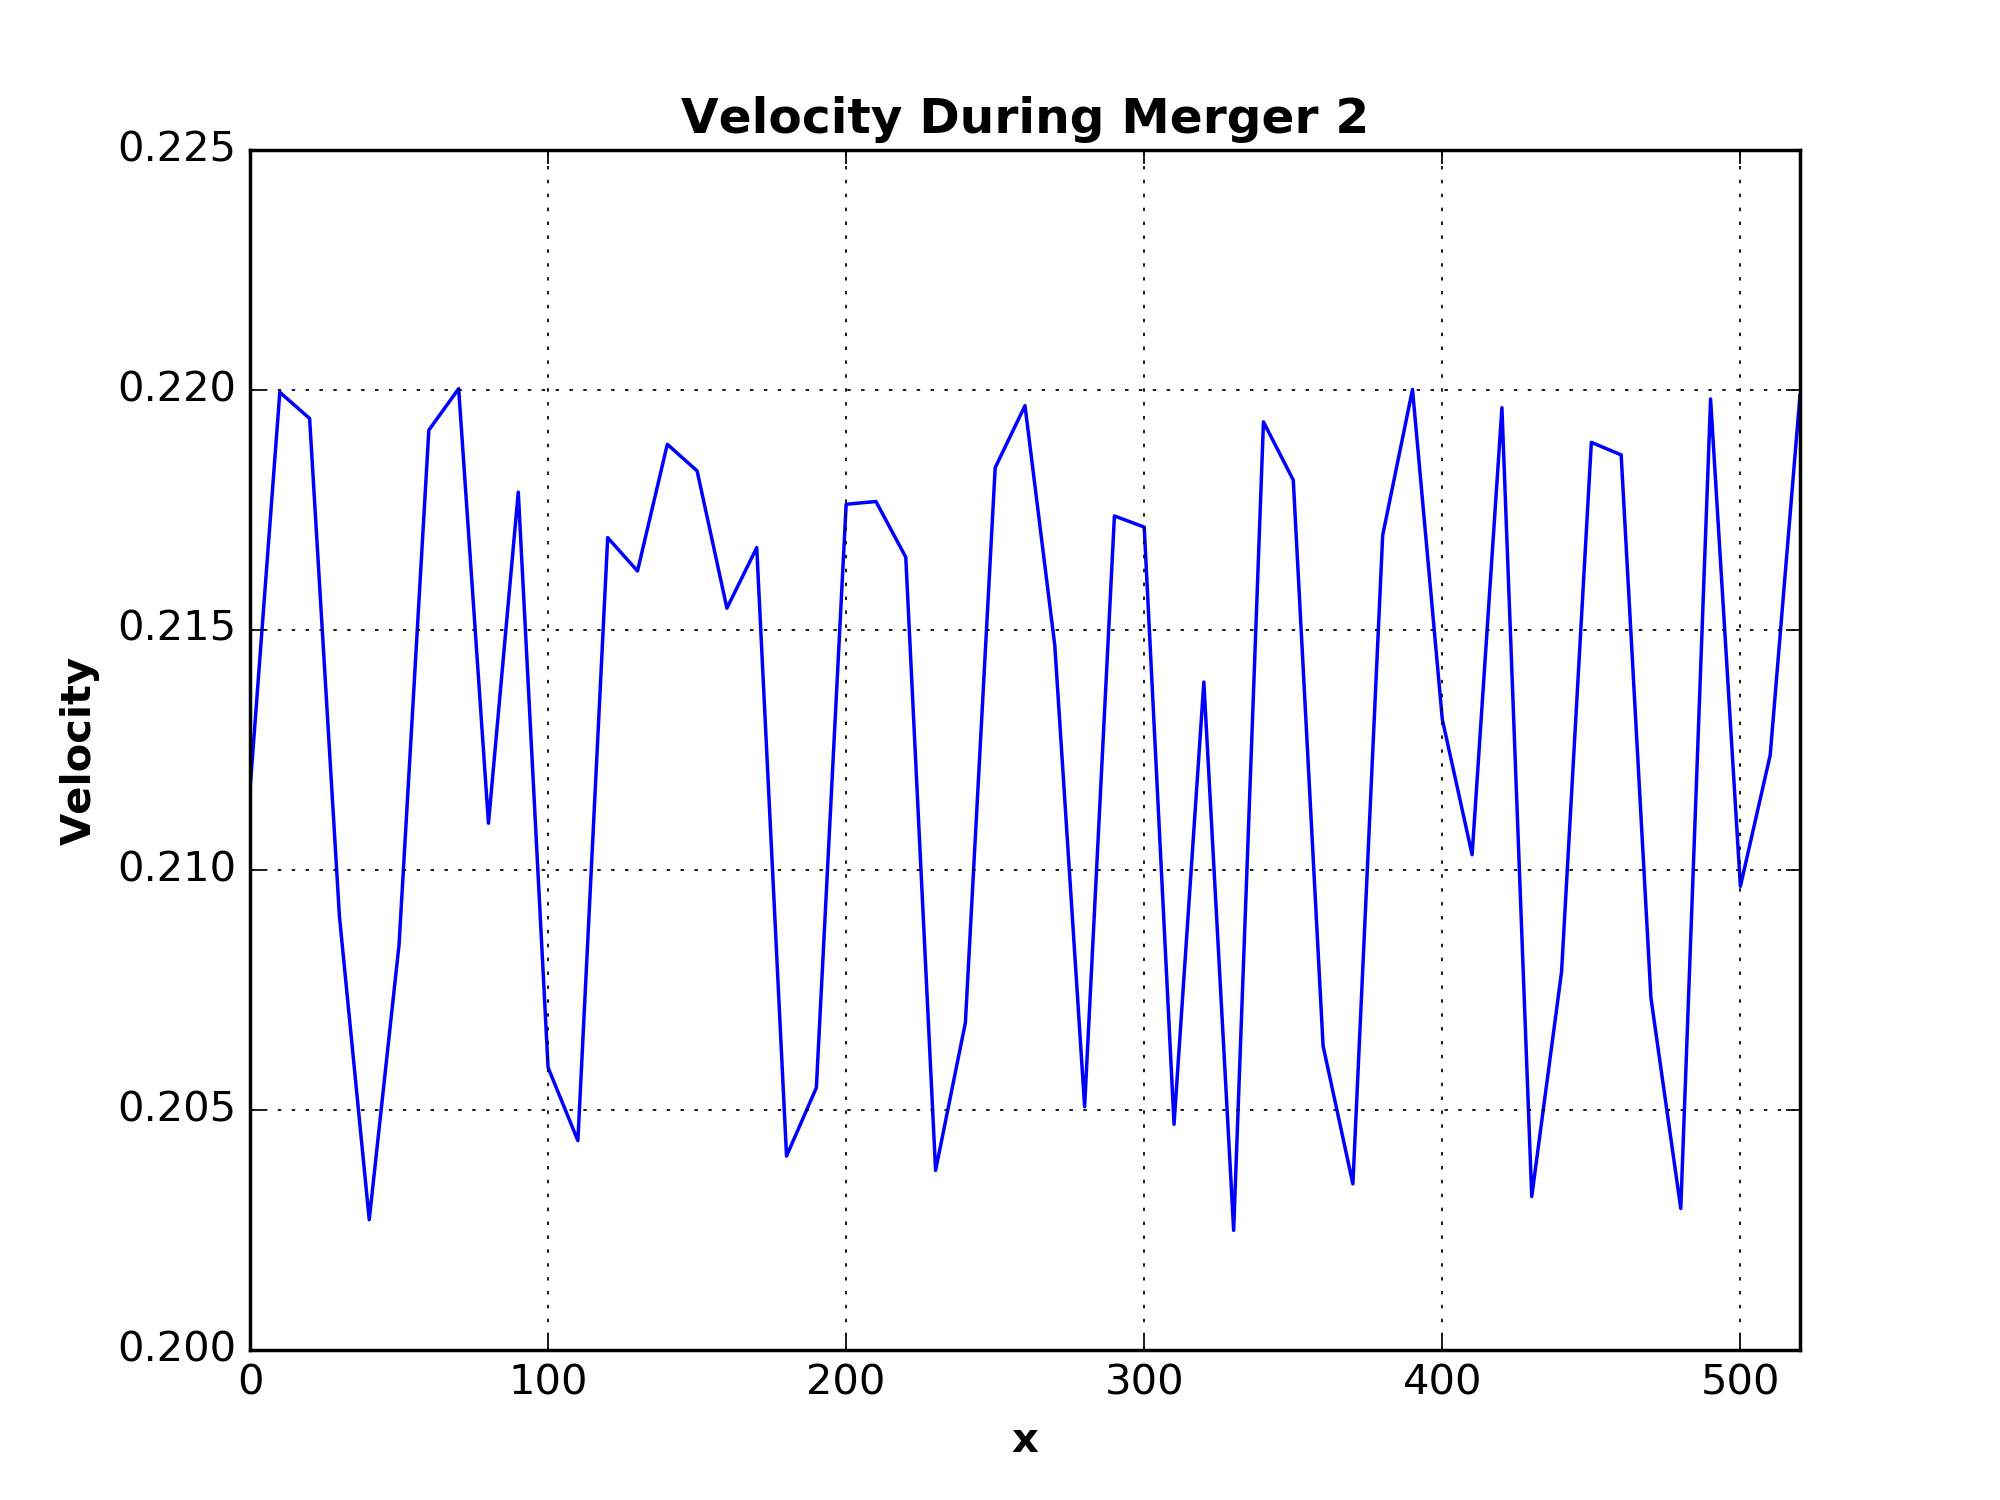
\includegraphics[width=\linewidth]{velocity_merger2.png}
        \caption[]%
        {{The velocity of the x-position during the second merger.}}
        \label{fig:velocity_merger2}
    \end{subfigure} %
    \caption[]
        {The plots above illustrate the velocity in the x-direction during the duration of the mergers.} 
        \label{fig:velocity_of_mergers}
\end{figure}

\begin{figure}[H]
\centering 
    \begin{subfigure}[b]{.475\textwidth}
        \centering
        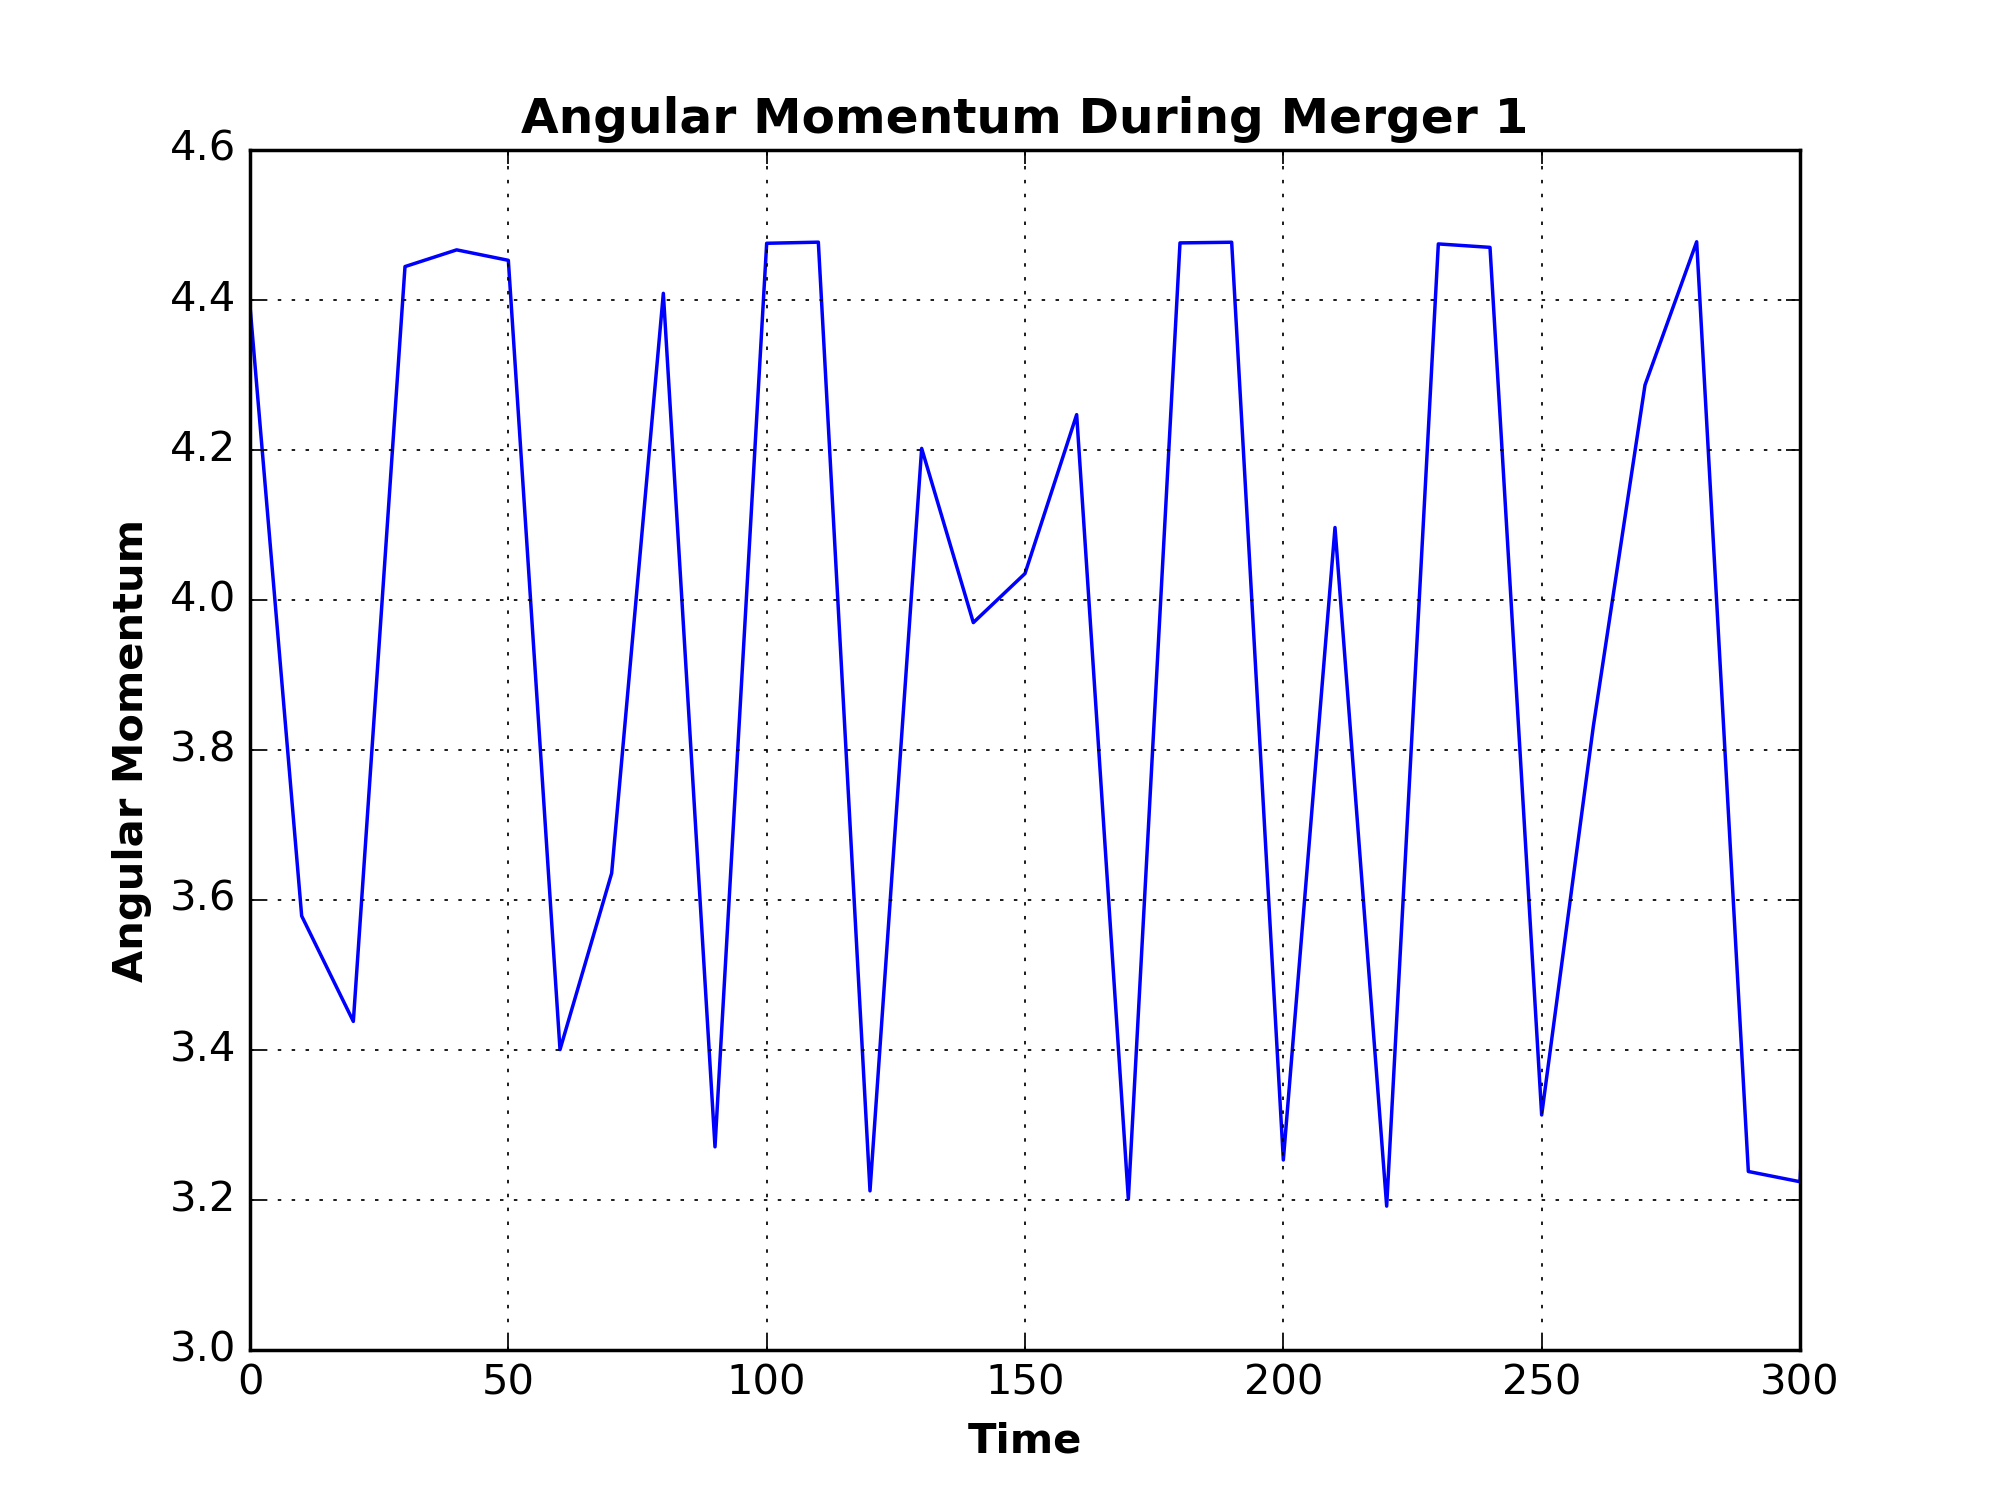
\includegraphics[width=\linewidth]{angular_momentum_merg13.png}
        \caption[]%
        {{The angular momentum during the first merger.}}
    
        \label{fig:ang_merger1}
    \end{subfigure} %'
    \hfill
    \begin{subfigure}[b]{.475\textwidth}
        \centering
        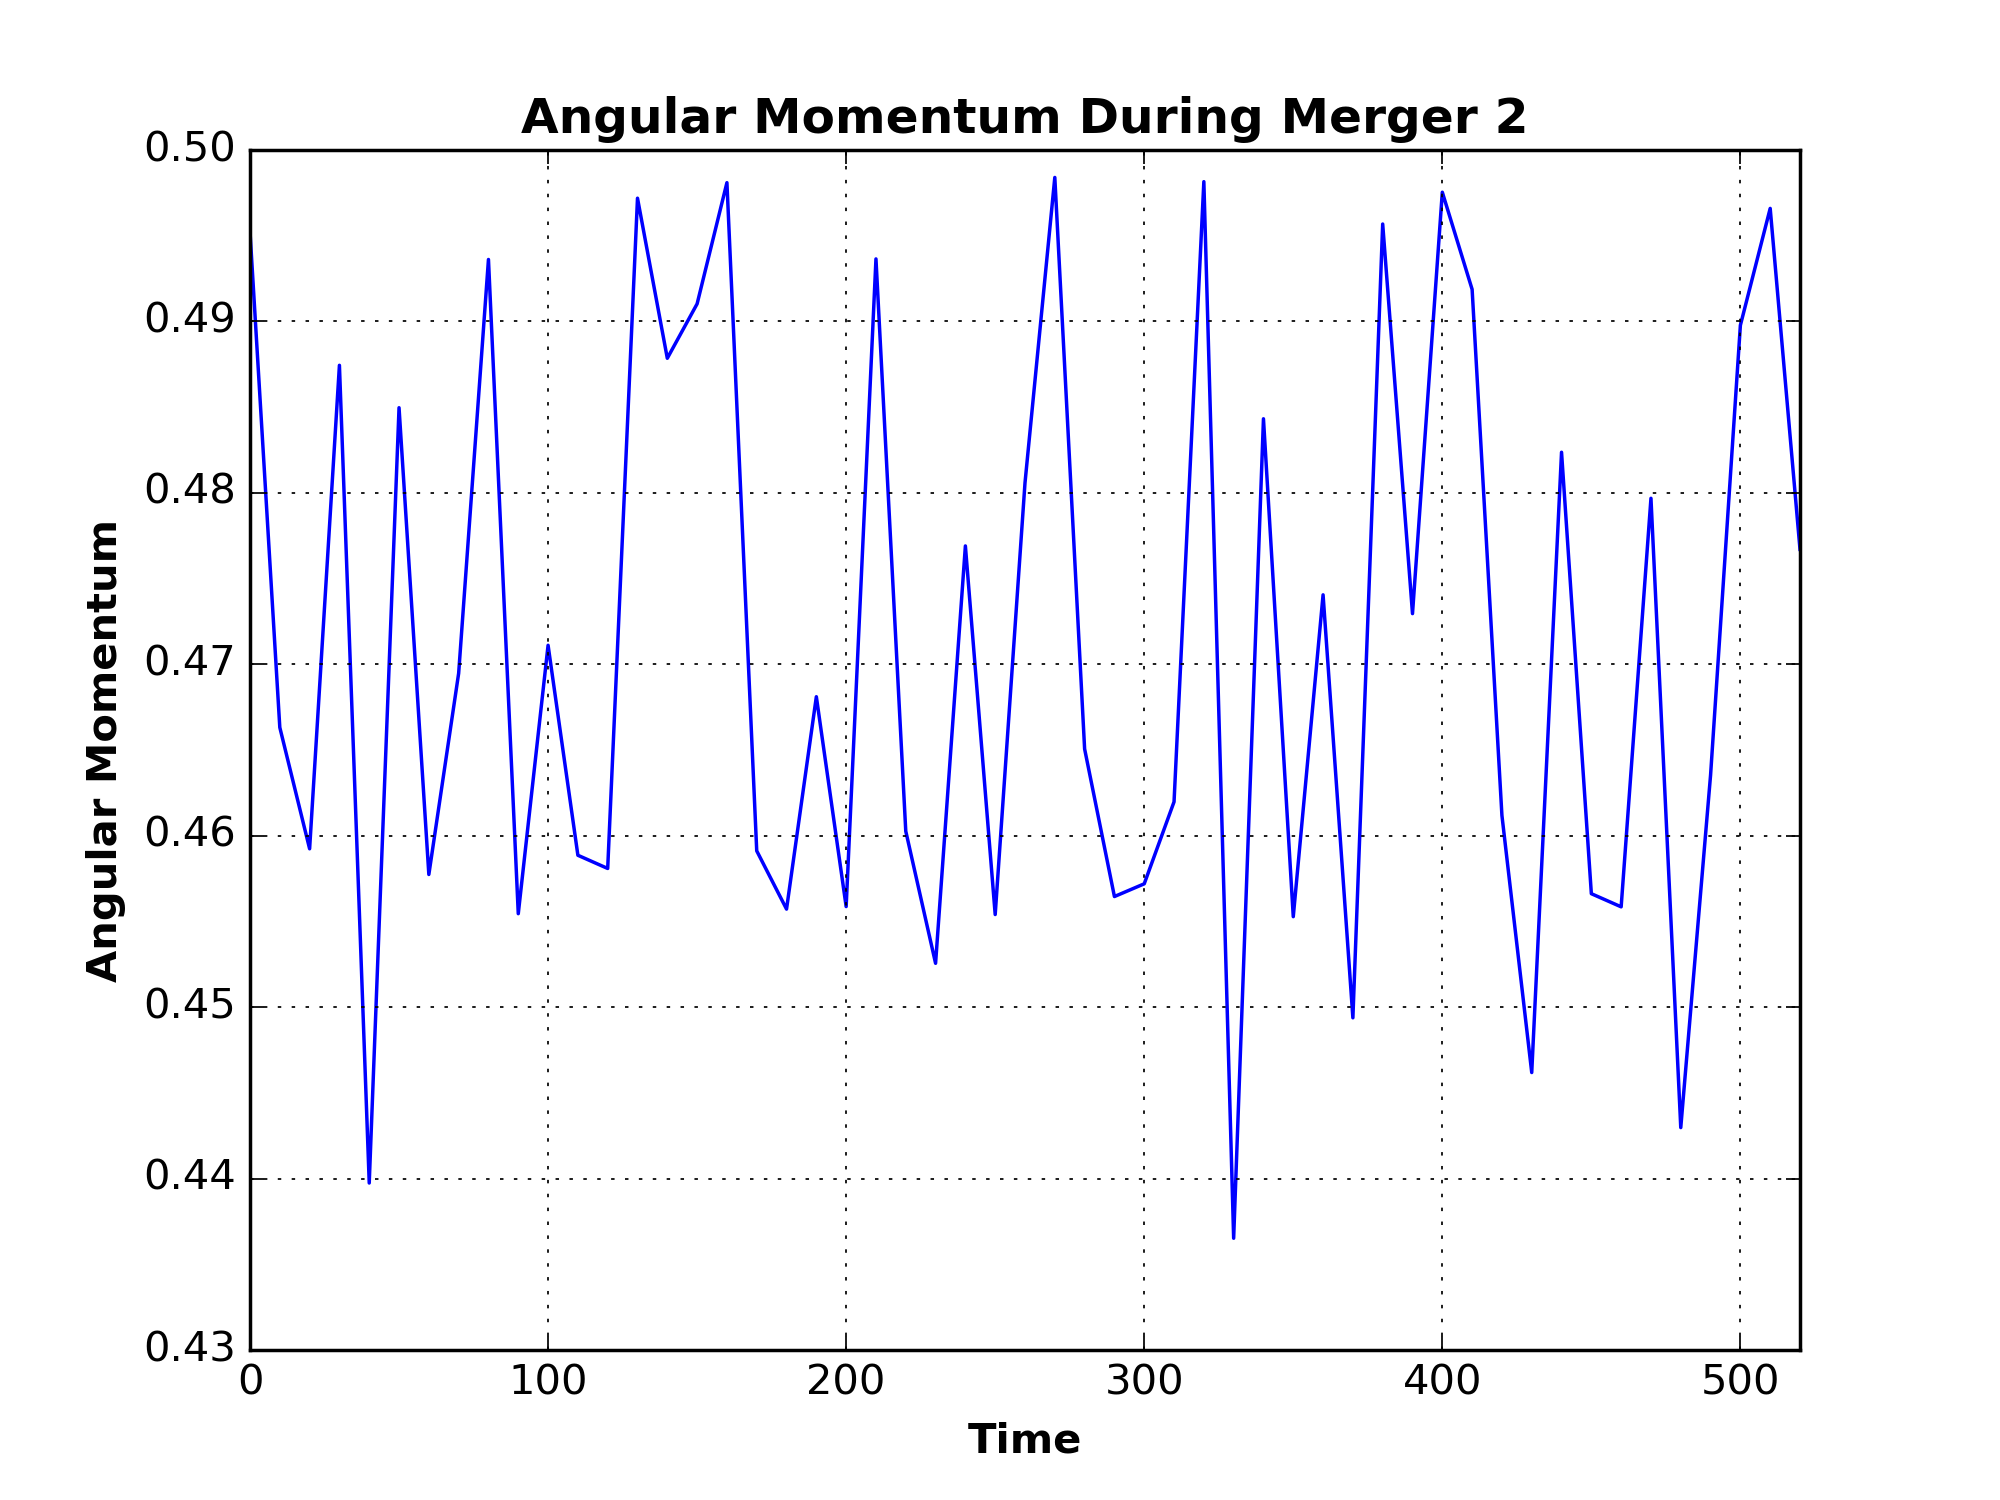
\includegraphics[width=\linewidth]{angular_momentum_merg21.png}
        \caption[]%
        {{The angular momentum during the second merger.}}
        \label{fig:ang_merger2} 
    \end{subfigure} %
    \caption[]
        {The plots above illustrate the total angular momentum during the duration of the mergers.} 
        \label{fig:angular_mmentum}
\end{figure}

\section*{Conclusion}
\addcontentsline{toc}{section}{Conclusion}

In conclusion, the merging of two elliptical galaxies was explored.

\addcontentsline{toc}{section}{Bibliography}

\bibliographystyle{apj.bst}
\bibliography{bib}
\end{document}

